\section{Architettura}

In questa sezione descriviamo brevemente l'architettura del sistema \progetto.

L'architettura adottata è \gloss{event-driven}: ogni componente è isolato e asincrono,
e comunica interfacciandosi e scambiandosi messaggi tramite il broker Apache Kafka.

Il sistema si divide principalmente in tre insiemi di componenti:

\begin{itemize}
    \item Producers
    \item Gestore Personale
    \item Consumers
\end{itemize}

\subsection{Producers}
Il Producer è il componente che resta in ascolto degli webhook provenienti dal suo applicativo specifico (e.g. Redmine, GitLab).
Ha lo scopo di immettere i messaggi su Kafka in formato JSON, conservando solo i campi di interesse e aggiungendone eventualmente di propri.

Al momento della stesura di questo manuale, i Producer implementati sono due:
\begin{itemize}
    \item RedmineProducer
    \item GitlabProducer
\end{itemize}

% \begin{figure}[H]
%     \centering
%     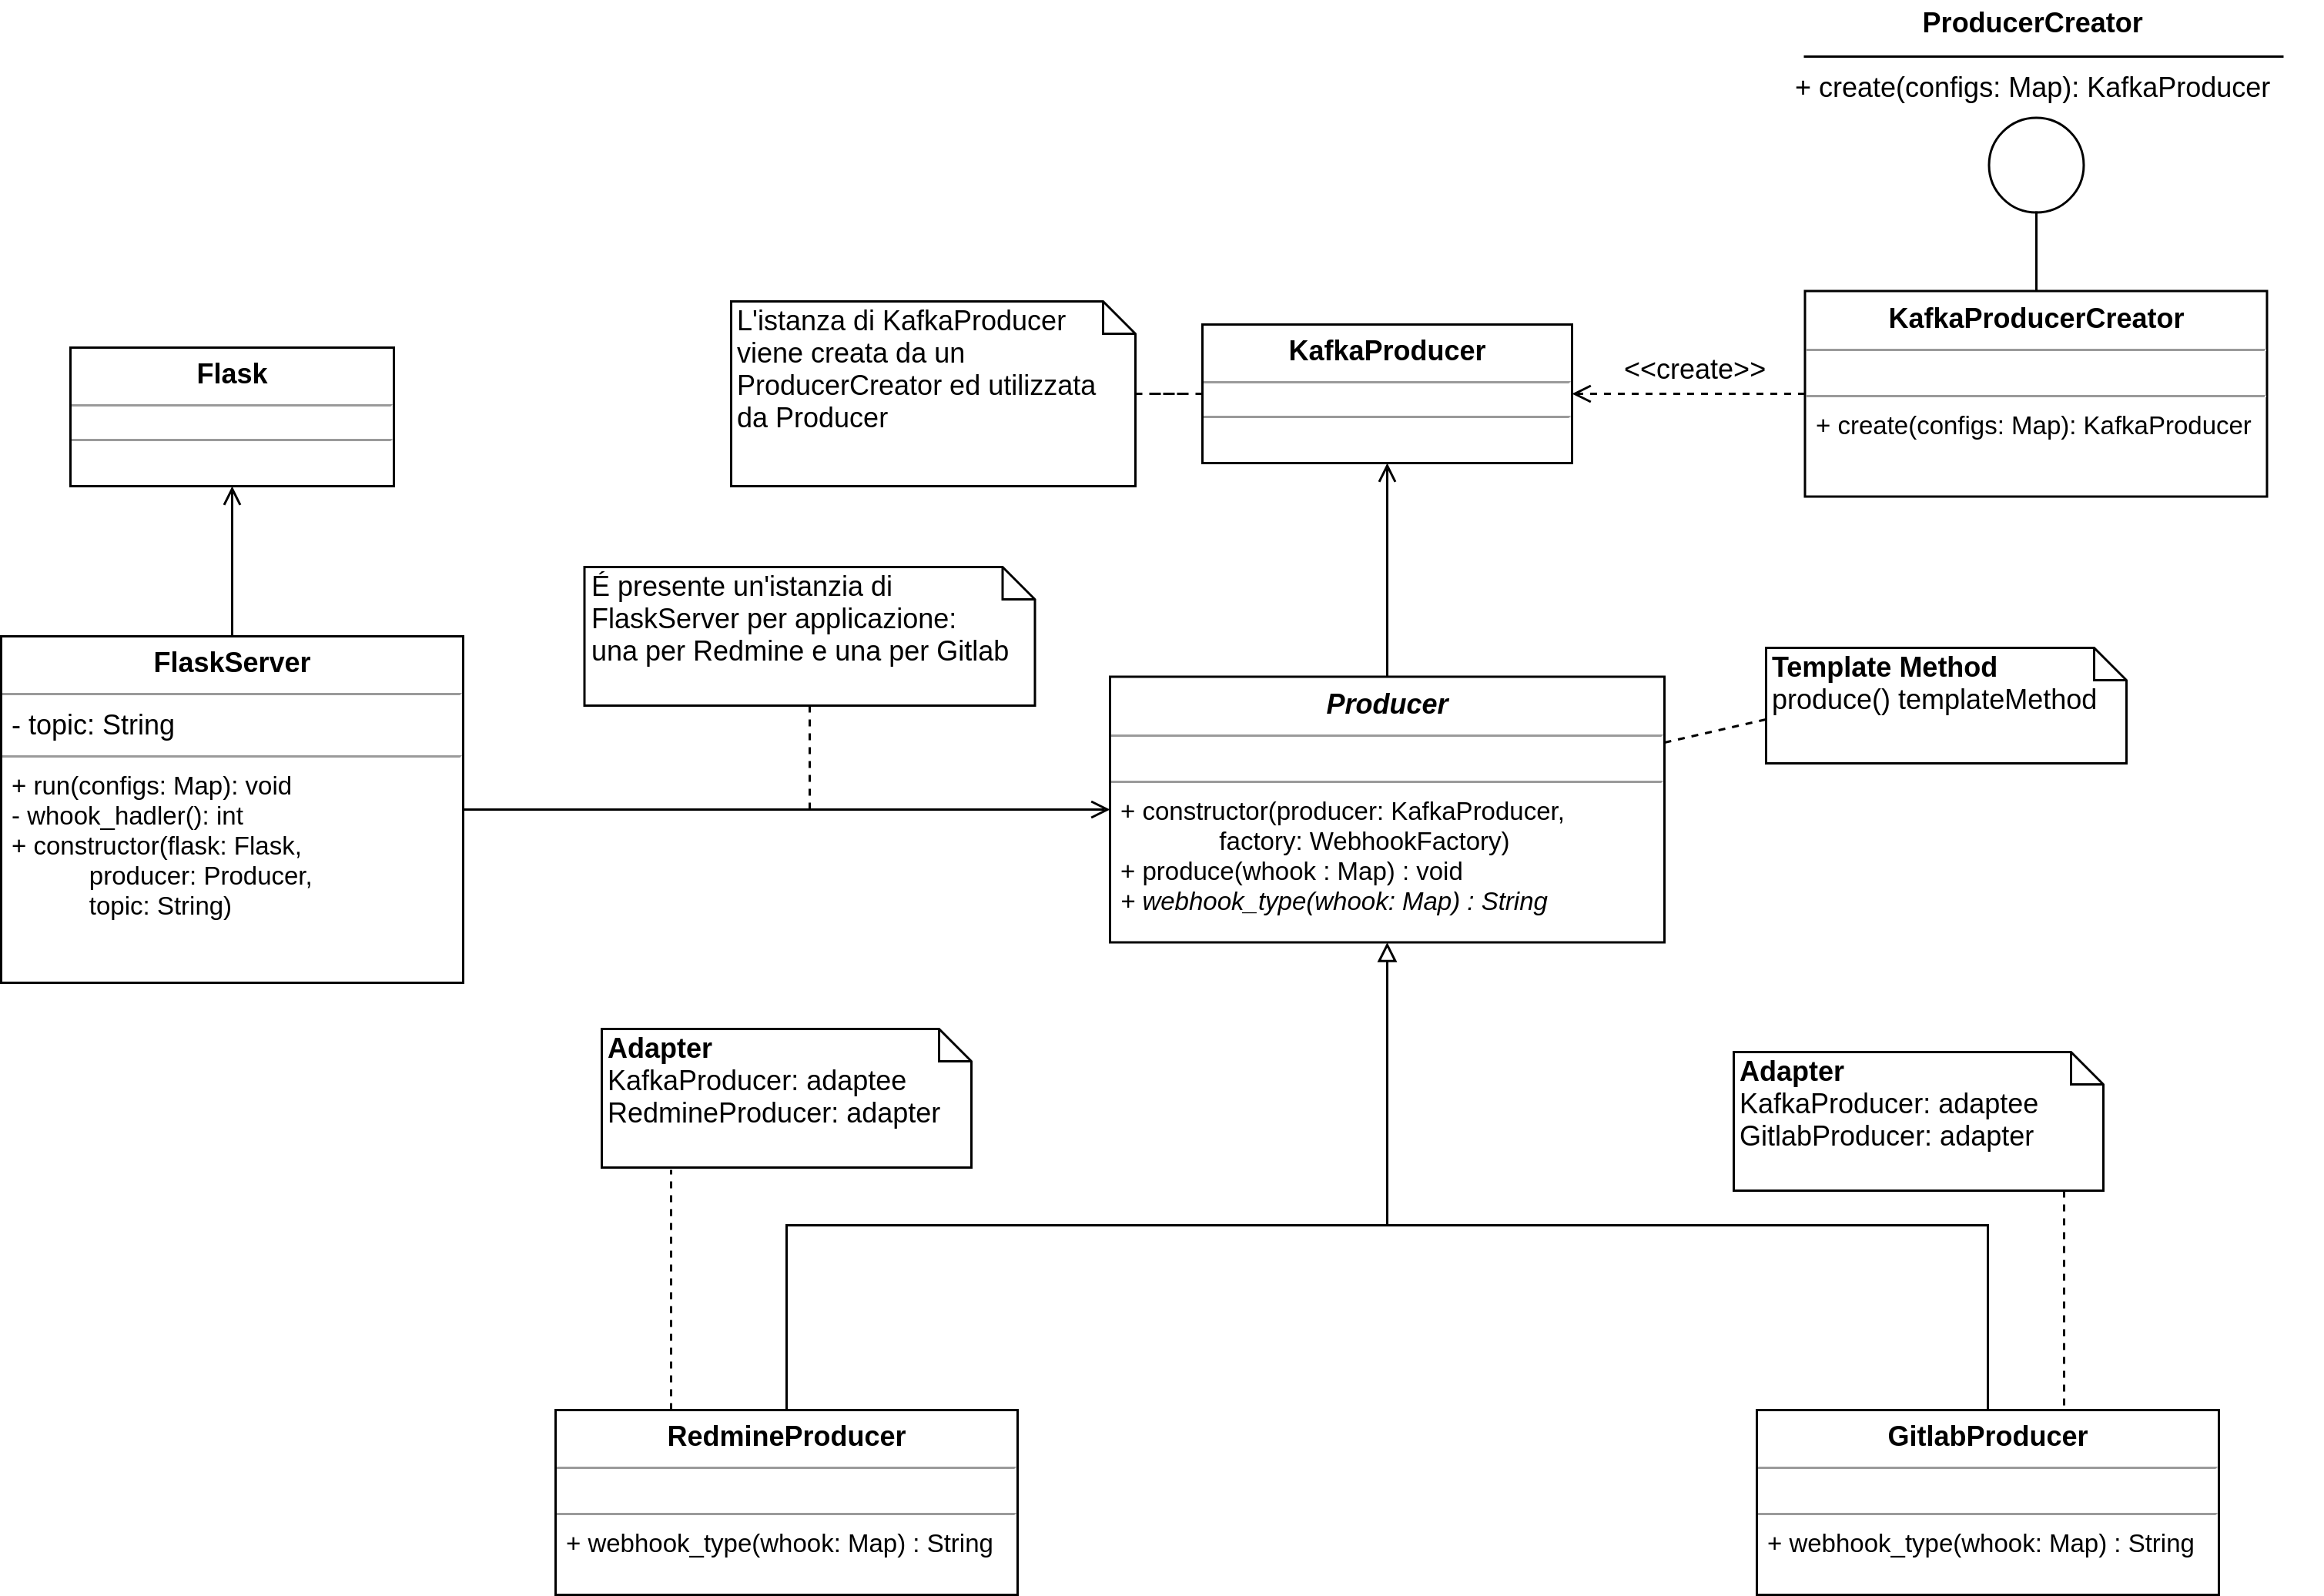
\includegraphics[width=\textwidth]{img/Producers.png}\\
%     \caption{Visione generale dei Producers}
%     \label{fig:producers}
% \end{figure}


\subsubsection{RedmineProducer}

\paragraph{Diagramma dei package}

\begin{figure}[H]
    \centering
    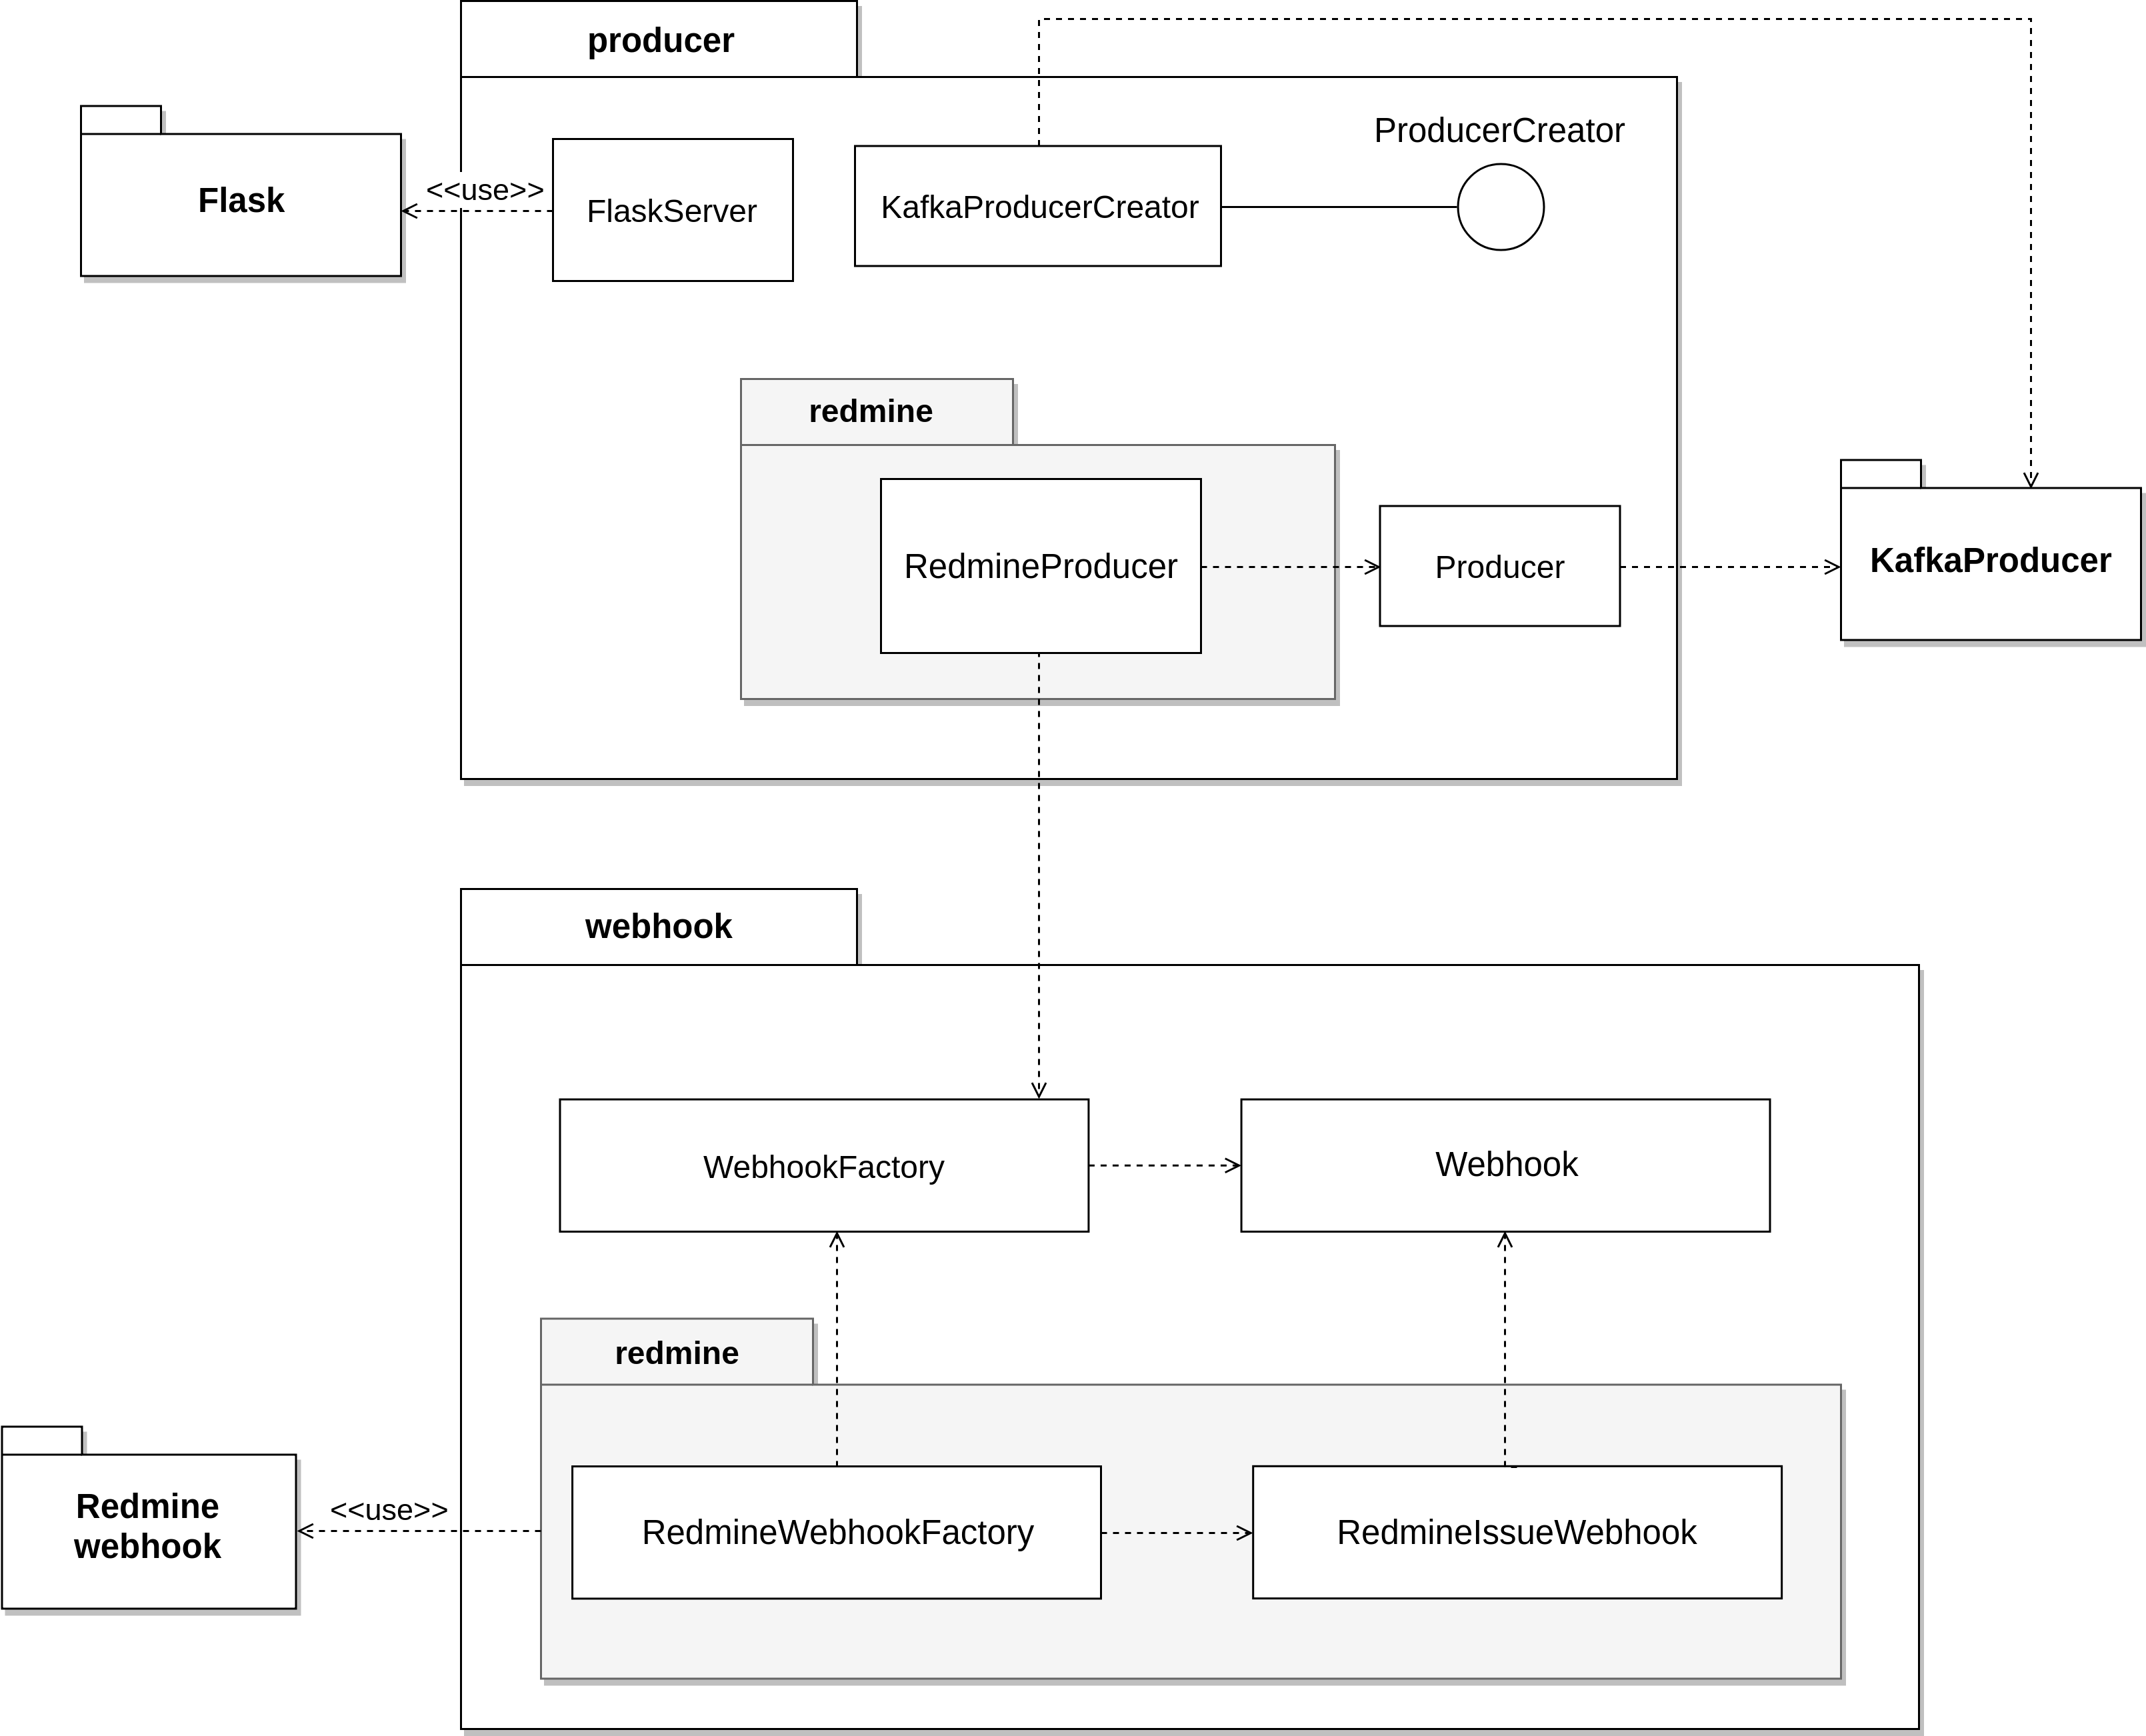
\includegraphics[width=\textwidth]{img/Package-RedmineProducer.png}\\
    \caption{Diagramma dei package di RedmineProducer}
    % \label{fig:producers}
\end{figure}

\paragraph{Diagramma delle classi}

\begin{figure}[H]
    \centering
    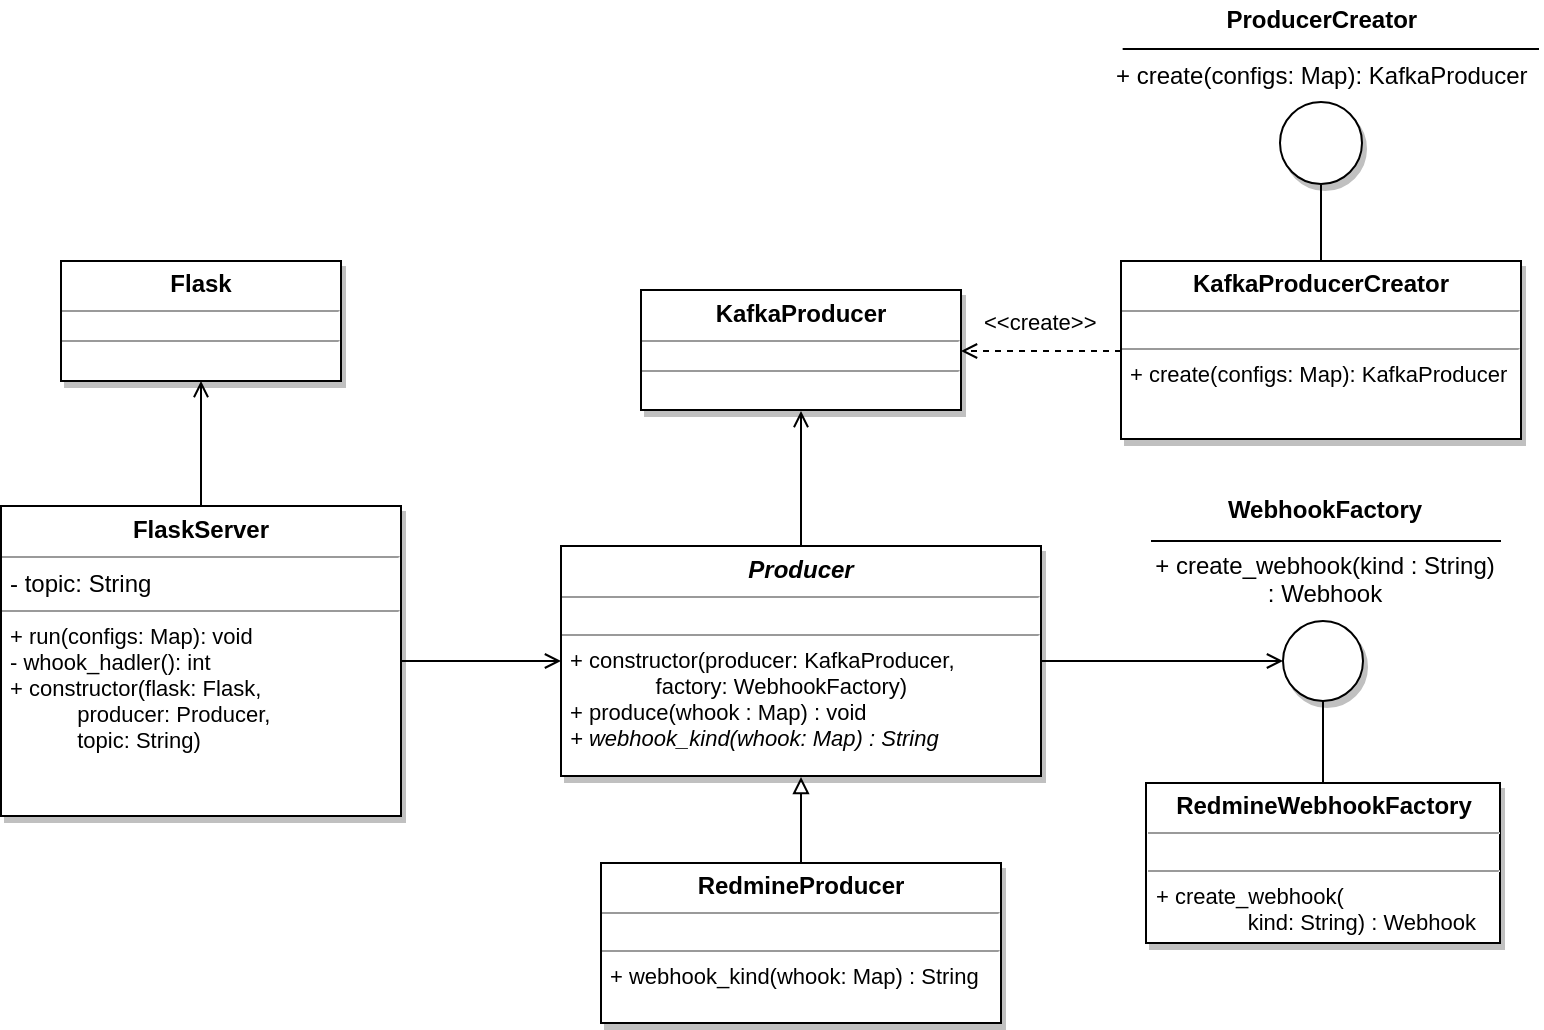
\includegraphics[width=\textwidth]{img/Producers-RedmineProducer.png}\\
    \caption{Diagramma delle classi di RedmineProducer}
    % \label{fig:producers}
\end{figure}

\begin{figure}[H]
    \centering
    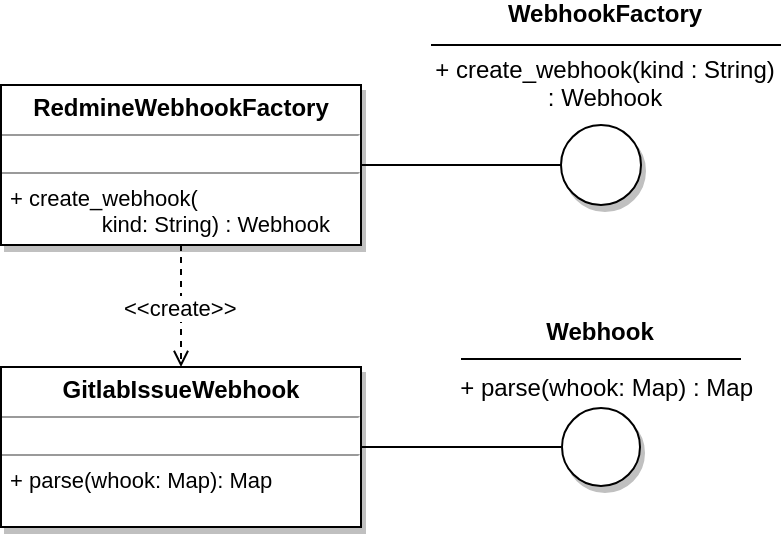
\includegraphics[width=0.6\textwidth]{img/Producers-RedmineWebhook.png}\\
    \caption{Diagramma delle classi di RedmineWebhookFactory}
    % \label{fig:producers}
\end{figure}



\subsubsection{GitlabProducer}

\paragraph{Diagramma dei package}

\begin{figure}[H]
    \centering
    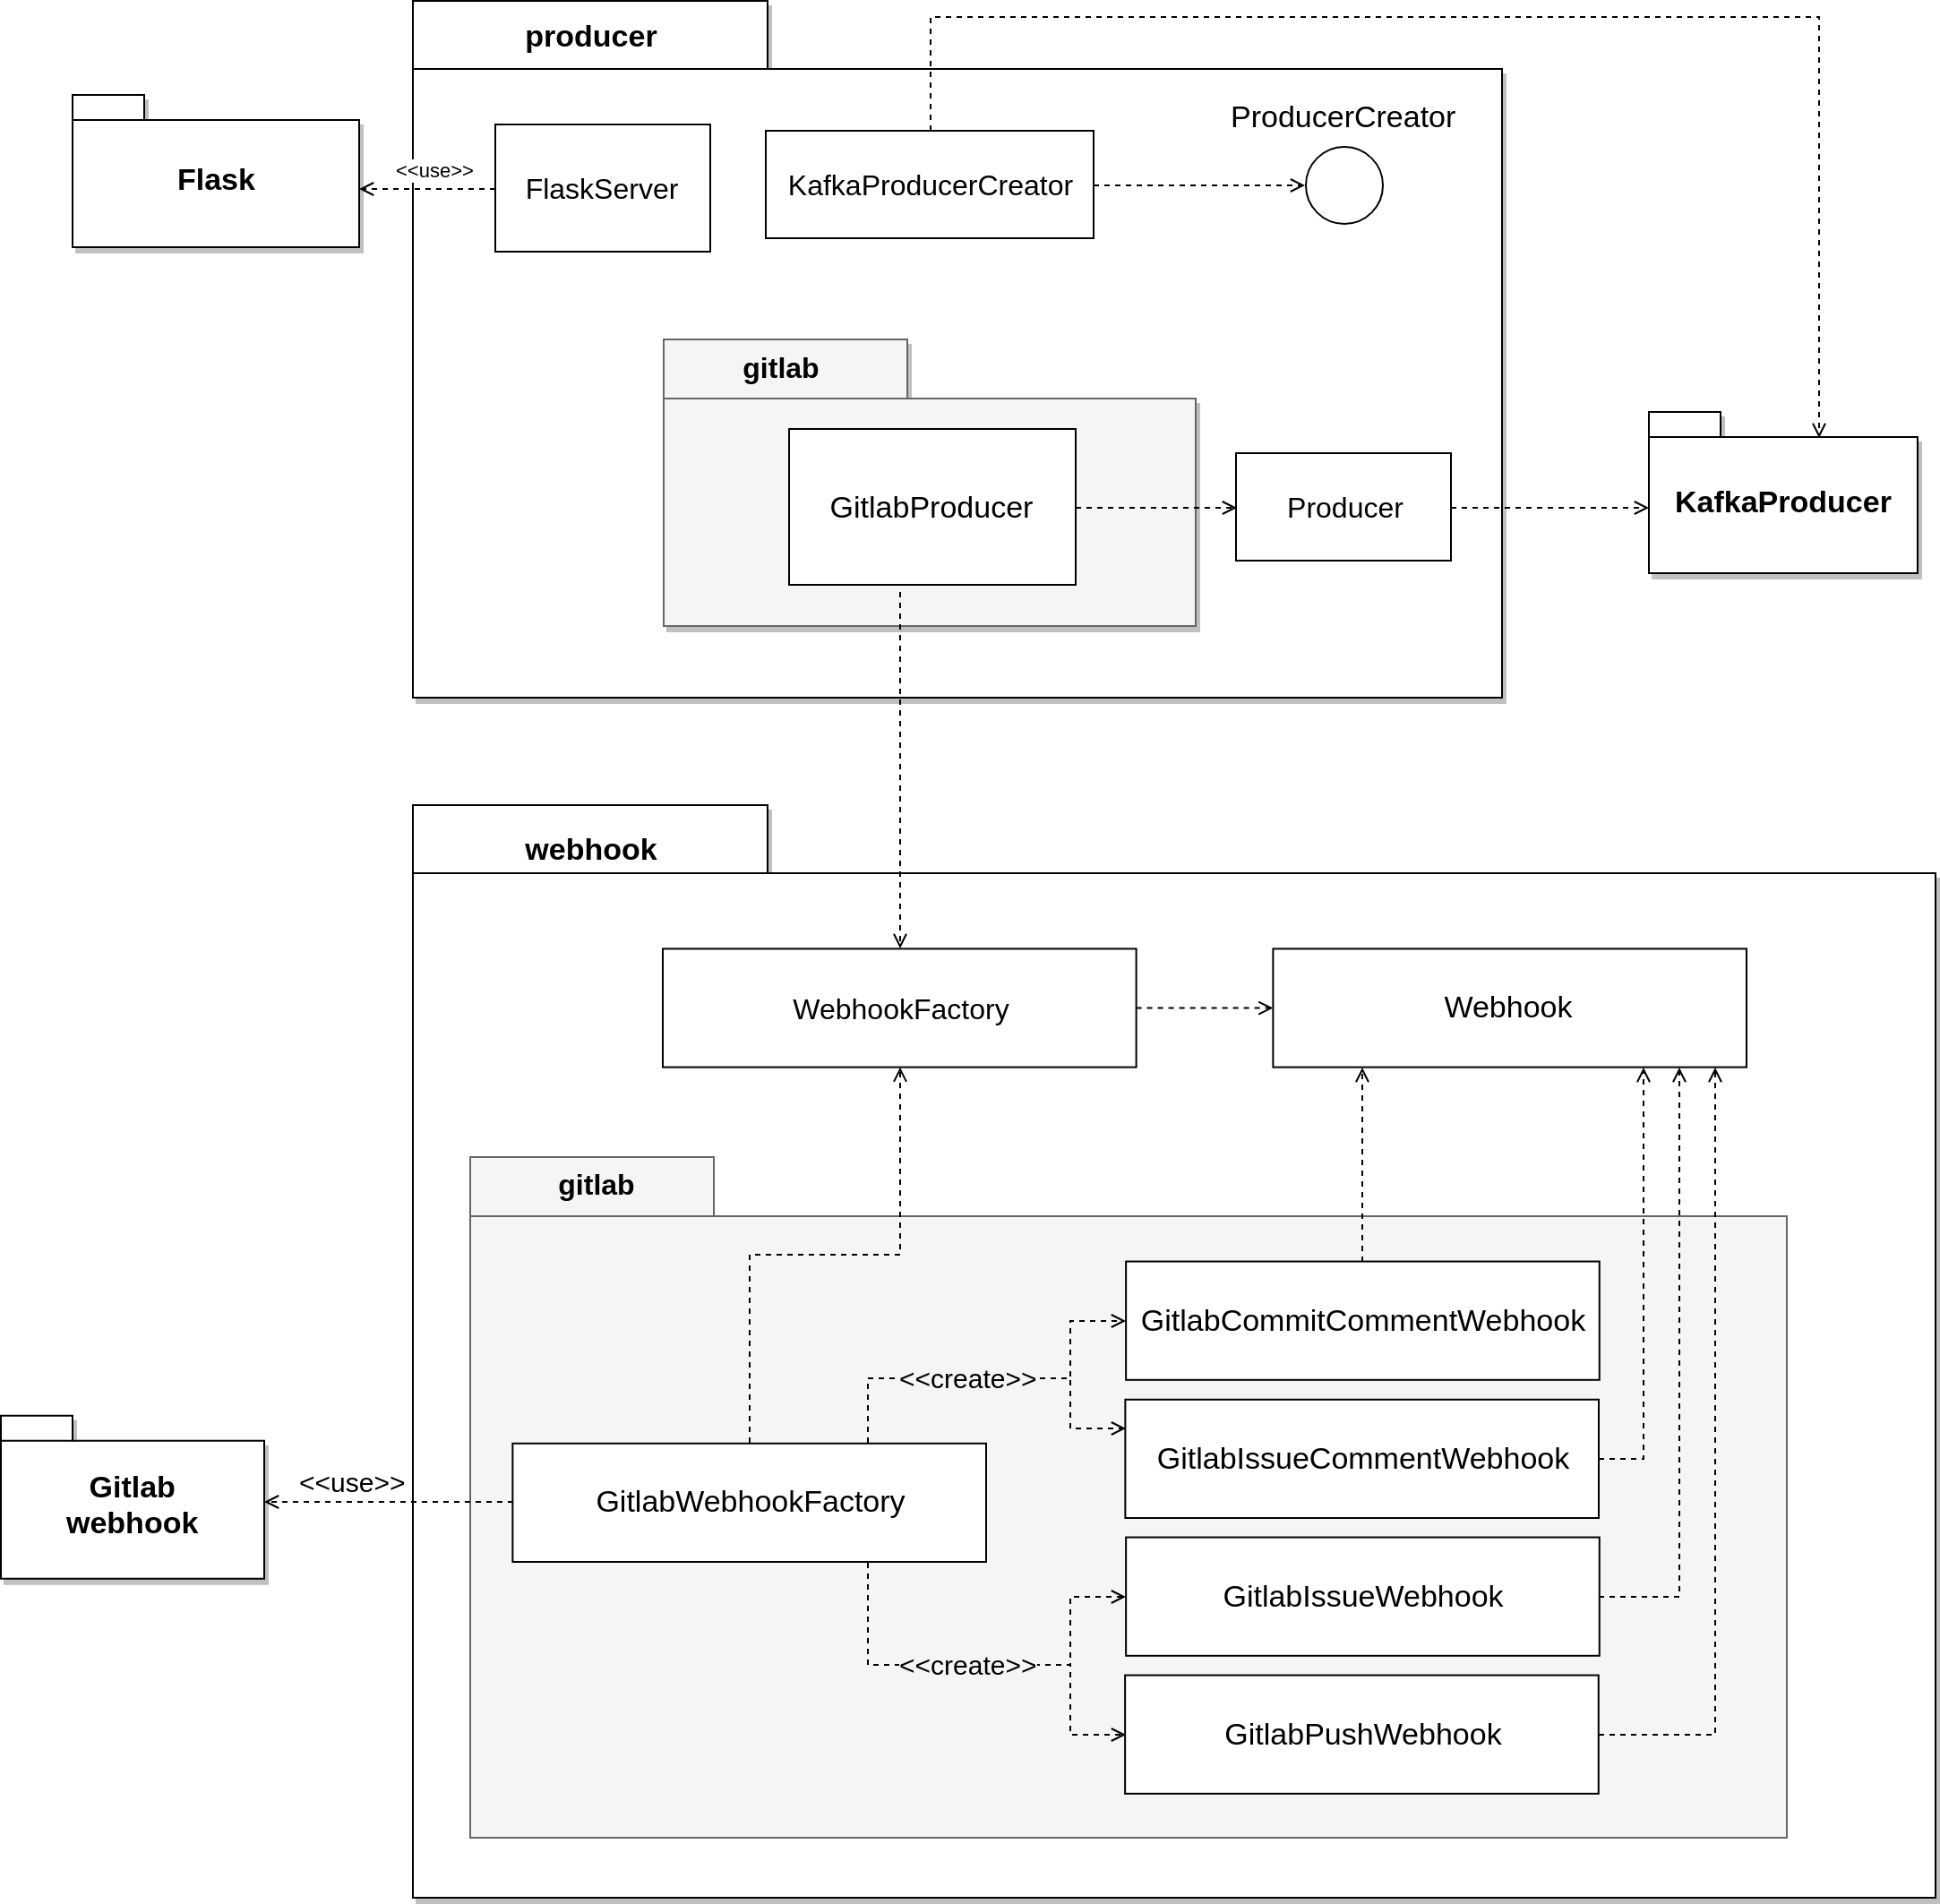
\includegraphics[width=\textwidth]{img/Package-GitLabProducer.png}\\
    \caption{Diagramma dei package di GitlabProducer}
    % \label{fig:producers}
\end{figure}


\paragraph{Diagramma delle classi}

\begin{figure}[H]
    \centering
    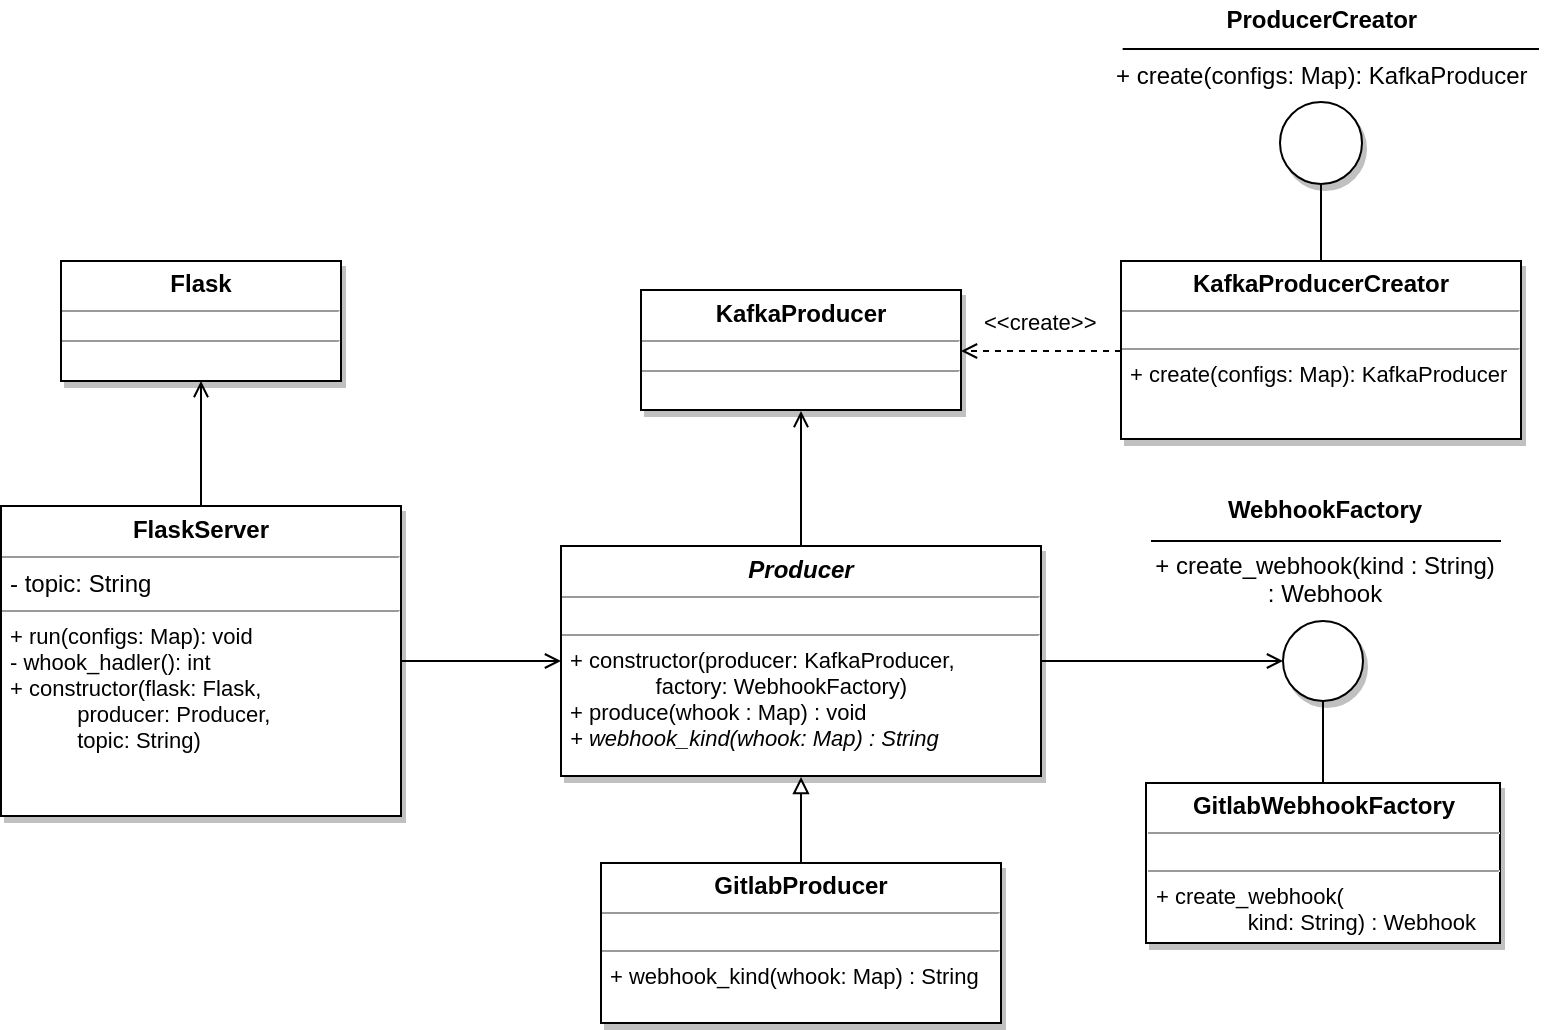
\includegraphics[width=\textwidth]{img/Producers-GitlabProducer.png}\\
    \caption{Diagramma delle classi di GitlabProducer}
    % \label{fig:producers}
\end{figure}


\begin{figure}[H]
    \centering
    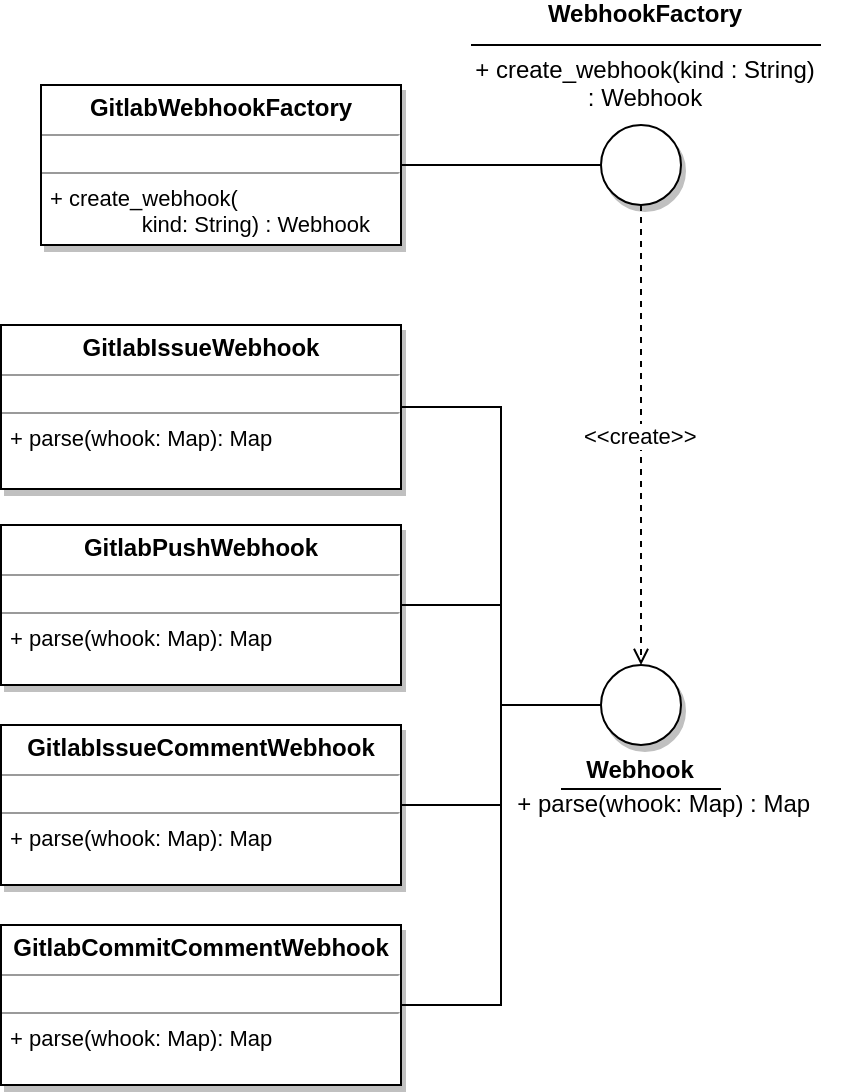
\includegraphics[width=0.6\textwidth]{img/Producers-GitlabWebhook.png}\\
    \caption{Diagramma delle classi di GitlabWebhookFactory}
    % \label{fig:producers}
\end{figure}



\subsection{Gestore Personale}
Il Gestore Personale è la componente con la logica più complessa del sistema Butterfly. Ha un proprio KafkaProducer e KafkaConsumer
che si occupano rispettivamente di ricevere i messaggi da Kafka e re-immetterli nelle code relative ai Consumer finali, passando per la logica
del personale, in cui ogni utente può selezionare i propri giorni di indisponibilità, la priorità dei progetti e la piattaforma di messaggistica sul
quale ricevere la notifica. Abbiamo pensato di dividerlo in tre parti per rendere tutto più chiaro.\newline
Questa prima parte riguarda la sezione del gestore personale che va a interfacciarsi con l’utente adottando un’architettura MVC pull model.
La view è pertanto totalmente passiva e l’unica cosa che fa è inoltrare i comandi ricevuti dall’utente all’\gloss{API REST}.

\subsubsection{Diagramma dei package}

\begin{figure}[H]
    \centering
    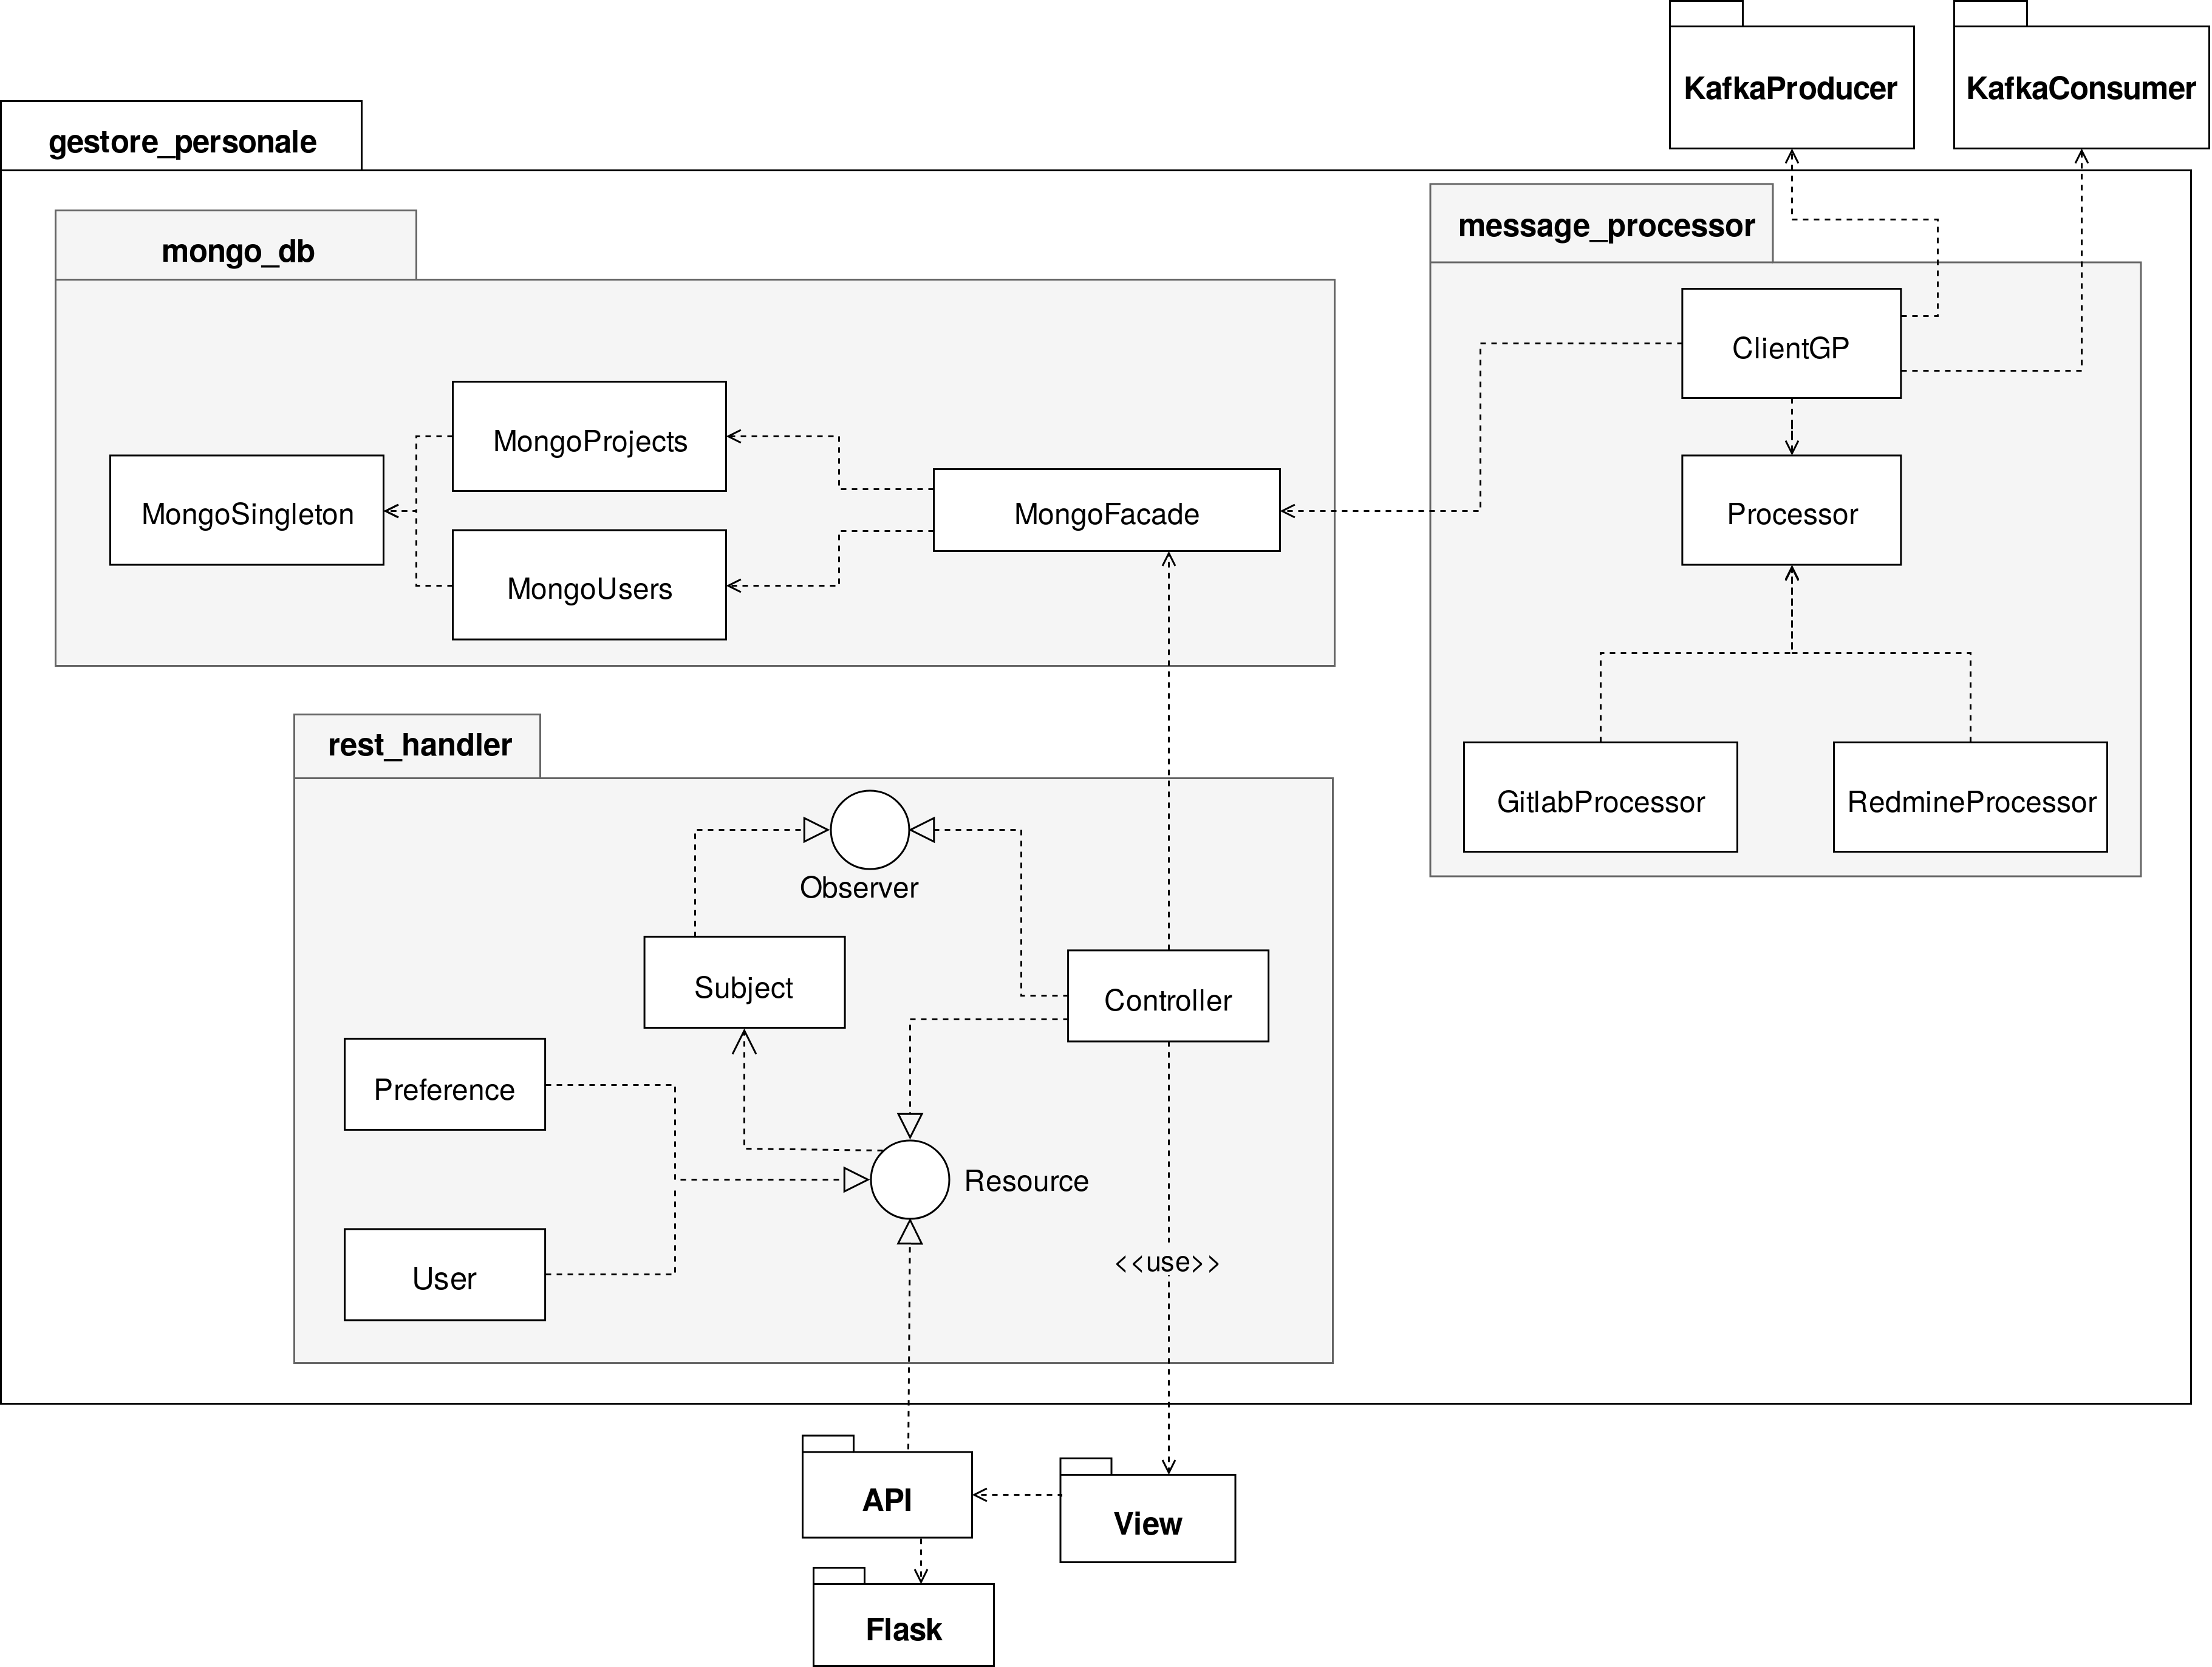
\includegraphics[width=\textwidth]{img/Package-GestorePersonale.png}\\
    \caption{Diagramma dei package del Gestore Personale}
    % \label{fig:GP-Processor}
\end{figure}


\begin{figure}[H]
    \centering
    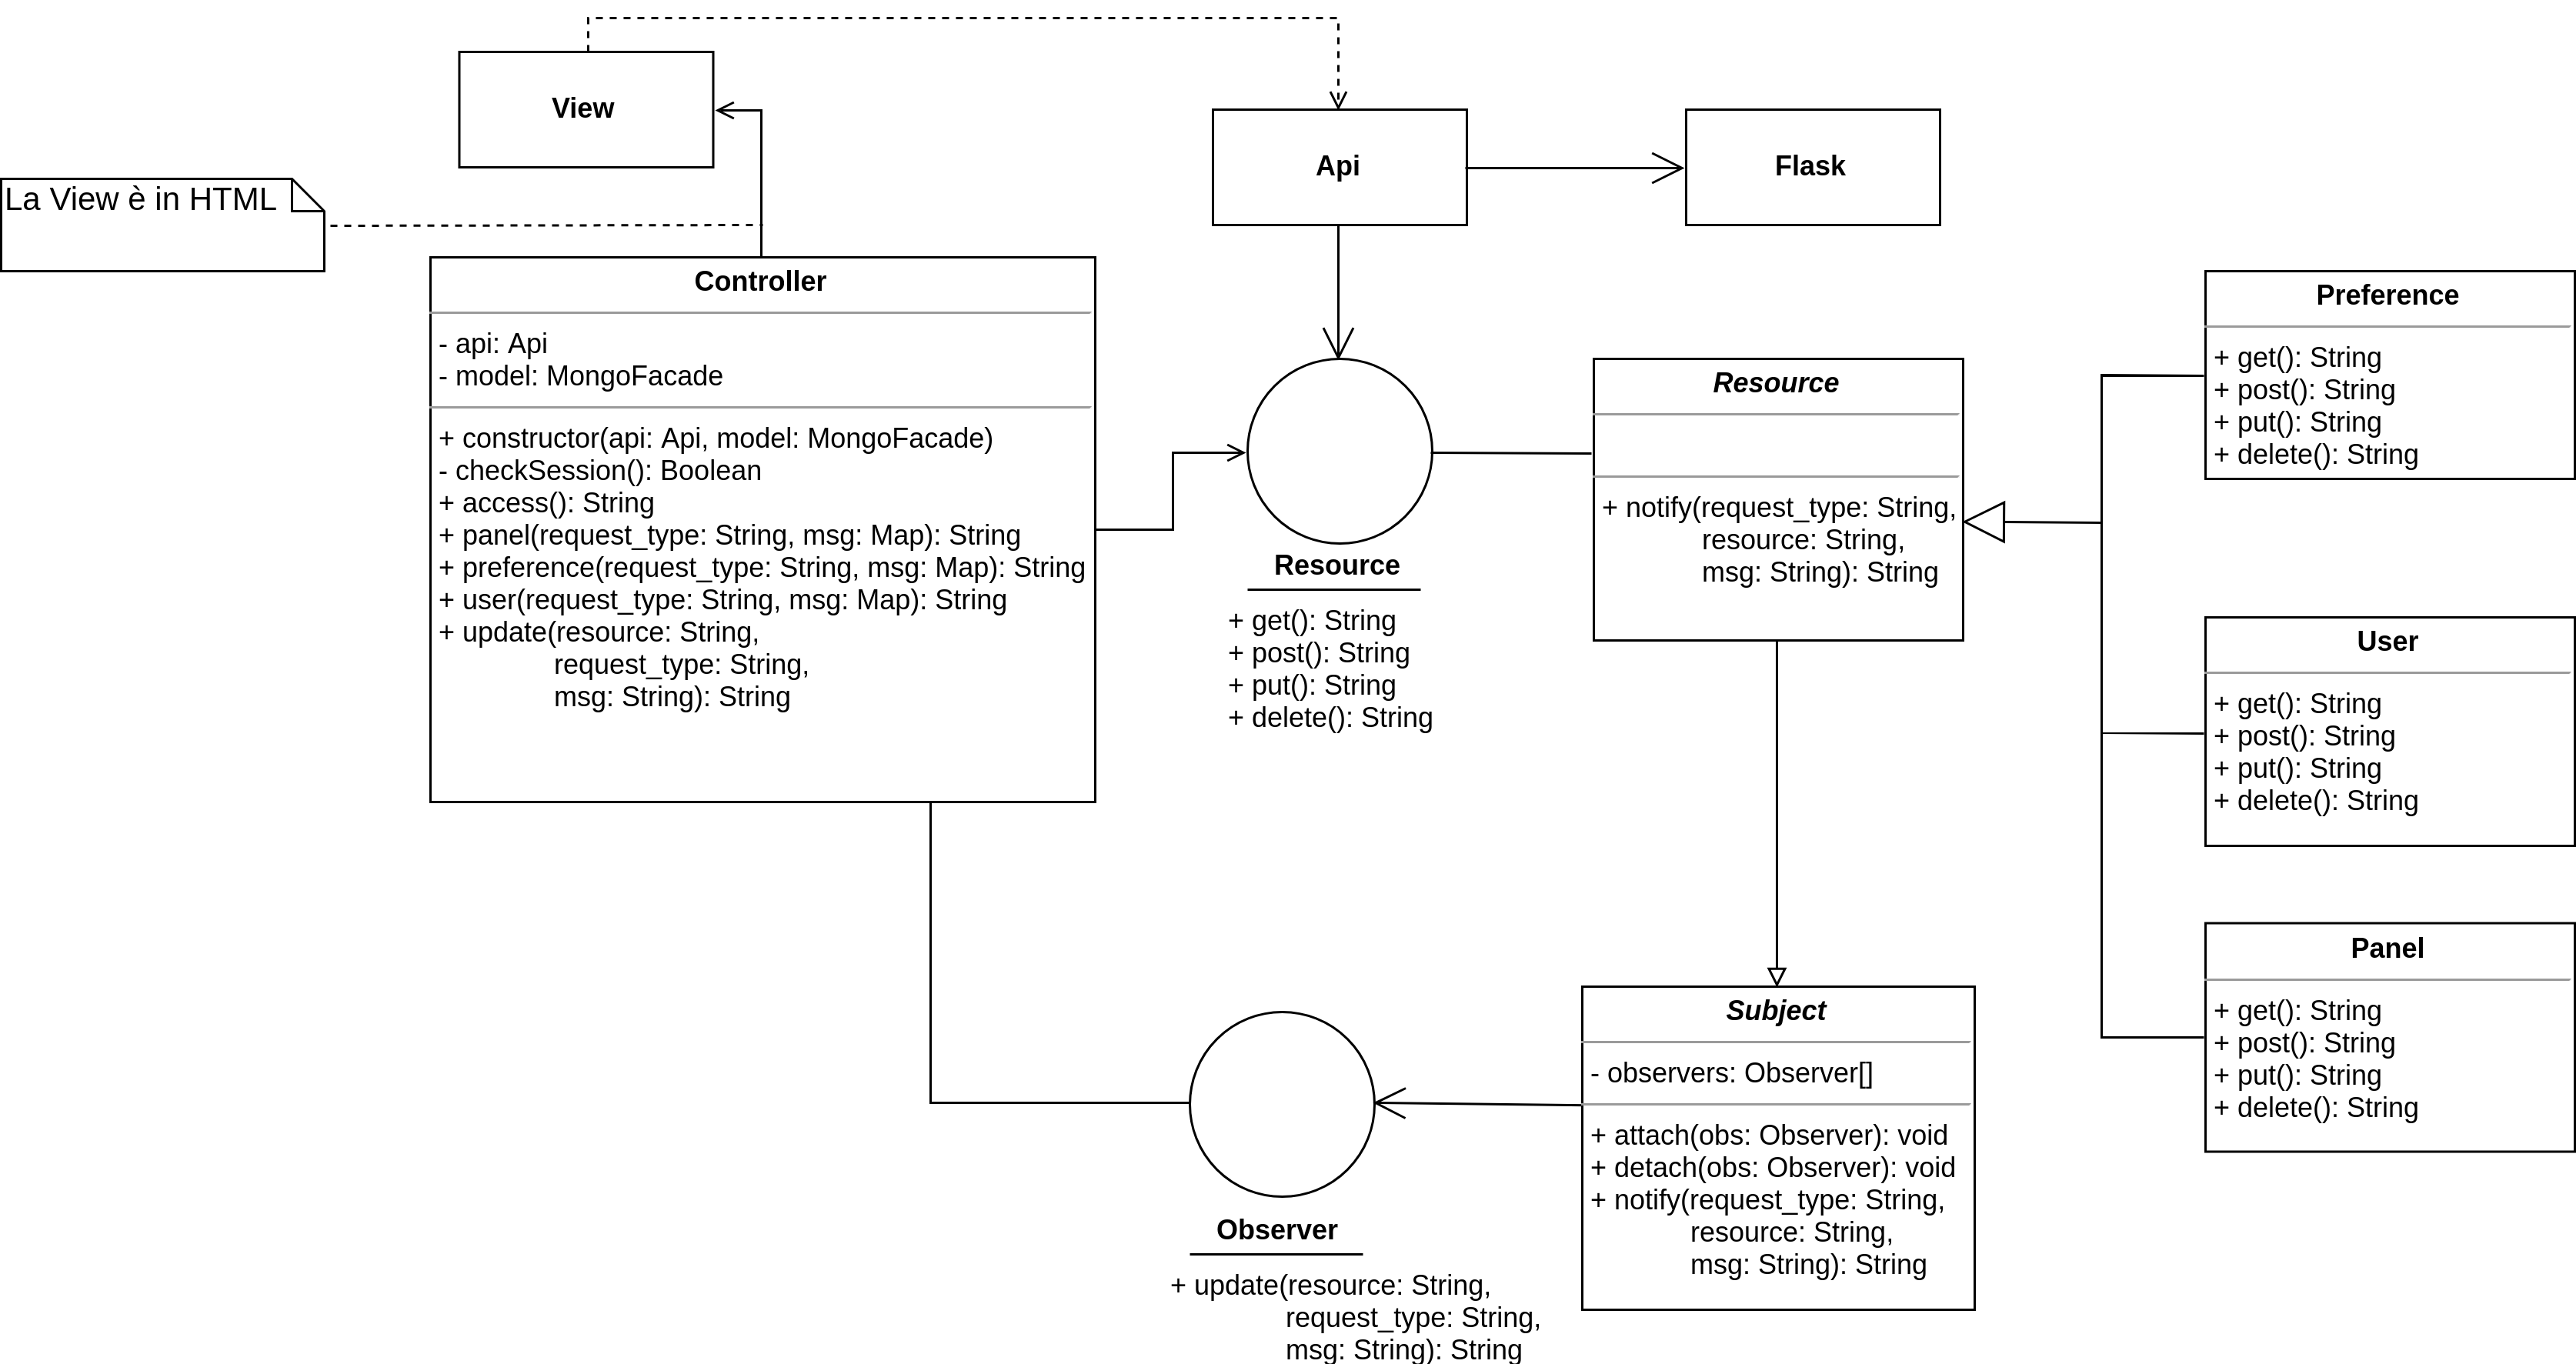
\includegraphics[width=\textwidth]{img/GP-Processor.png}\\
    \caption{Interfaccia del Gestore Personale}
    \label{fig:GP-Processor}
\end{figure}

Qua viene mostrato come il Gestore Personale si interfaccia con \gloss{MongoDB}, ovvero MongoUser e MongoProject. Sono suddivisi in base alla risorsa di interesse.

\begin{figure}[H]
    \centering
    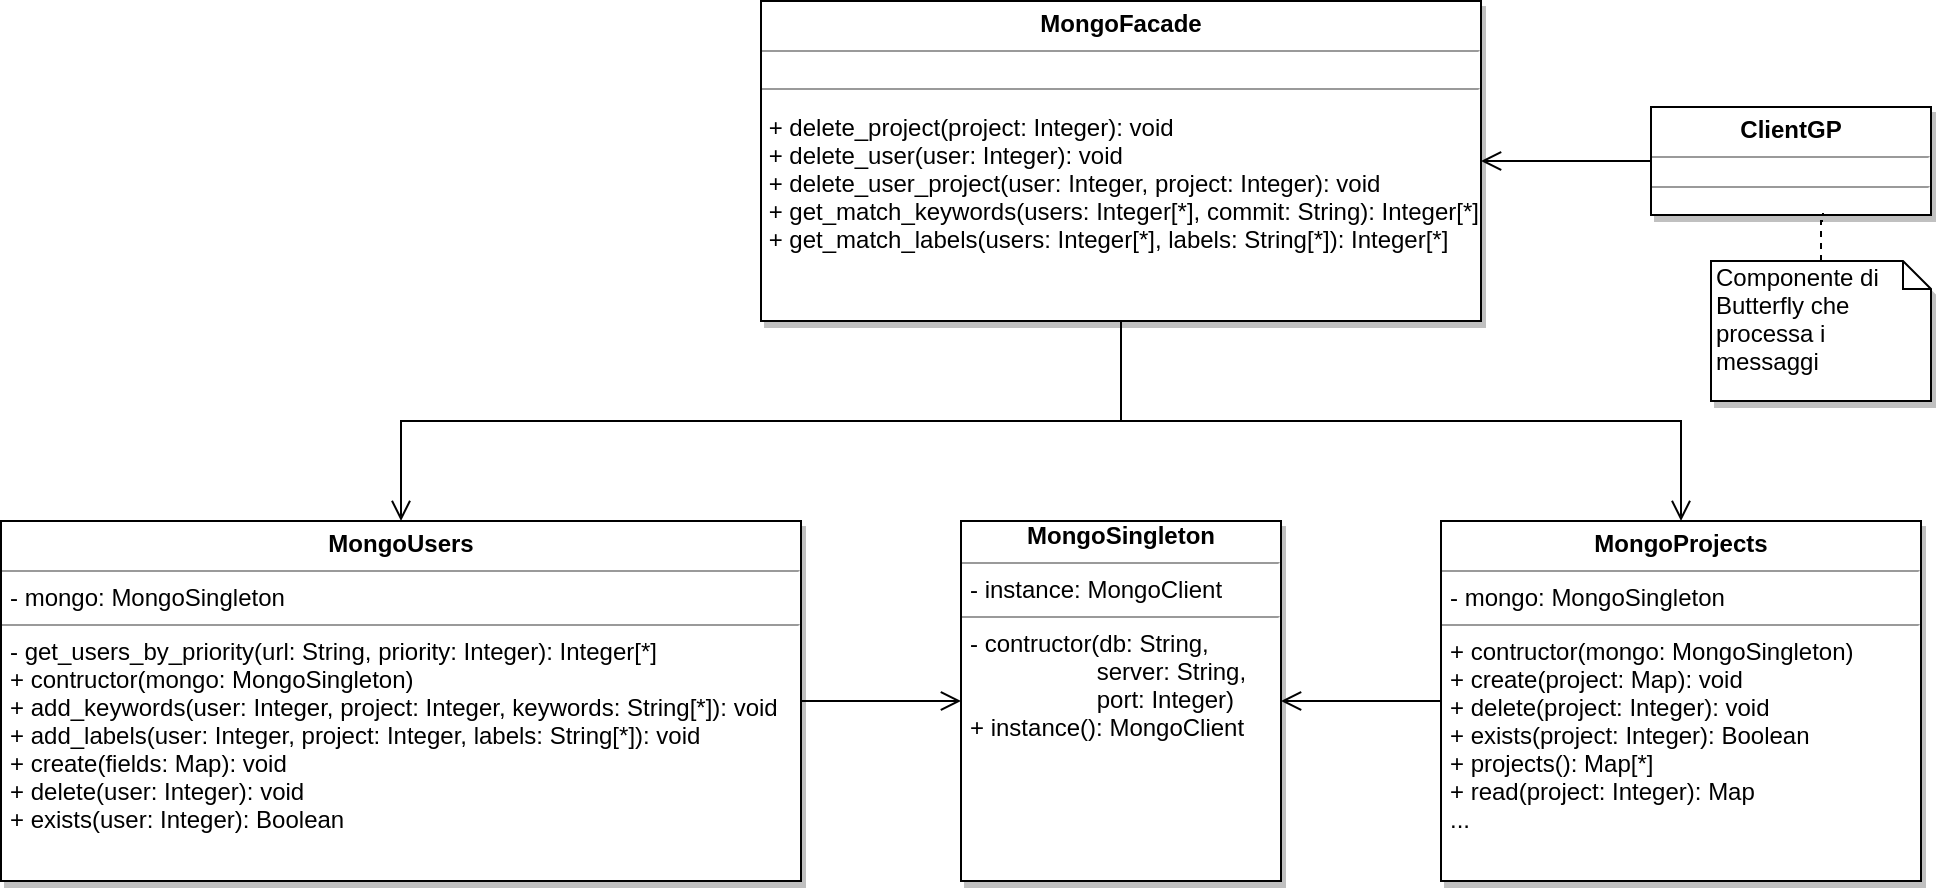
\includegraphics[width=\textwidth]{img/GP-Mongo.png}\\
    \caption{Interazione con MongoDB del Gestore Personale}
    \label{fig:GP-Mongo}
\end{figure}

Mentre in quest'ultima viene mostrato come il Gestore Personale si interfaccia con Kafka, questa riguarda il core del Gestore Personale, si occupa di processare
i messaggi

\begin{figure}[H]
    \centering
    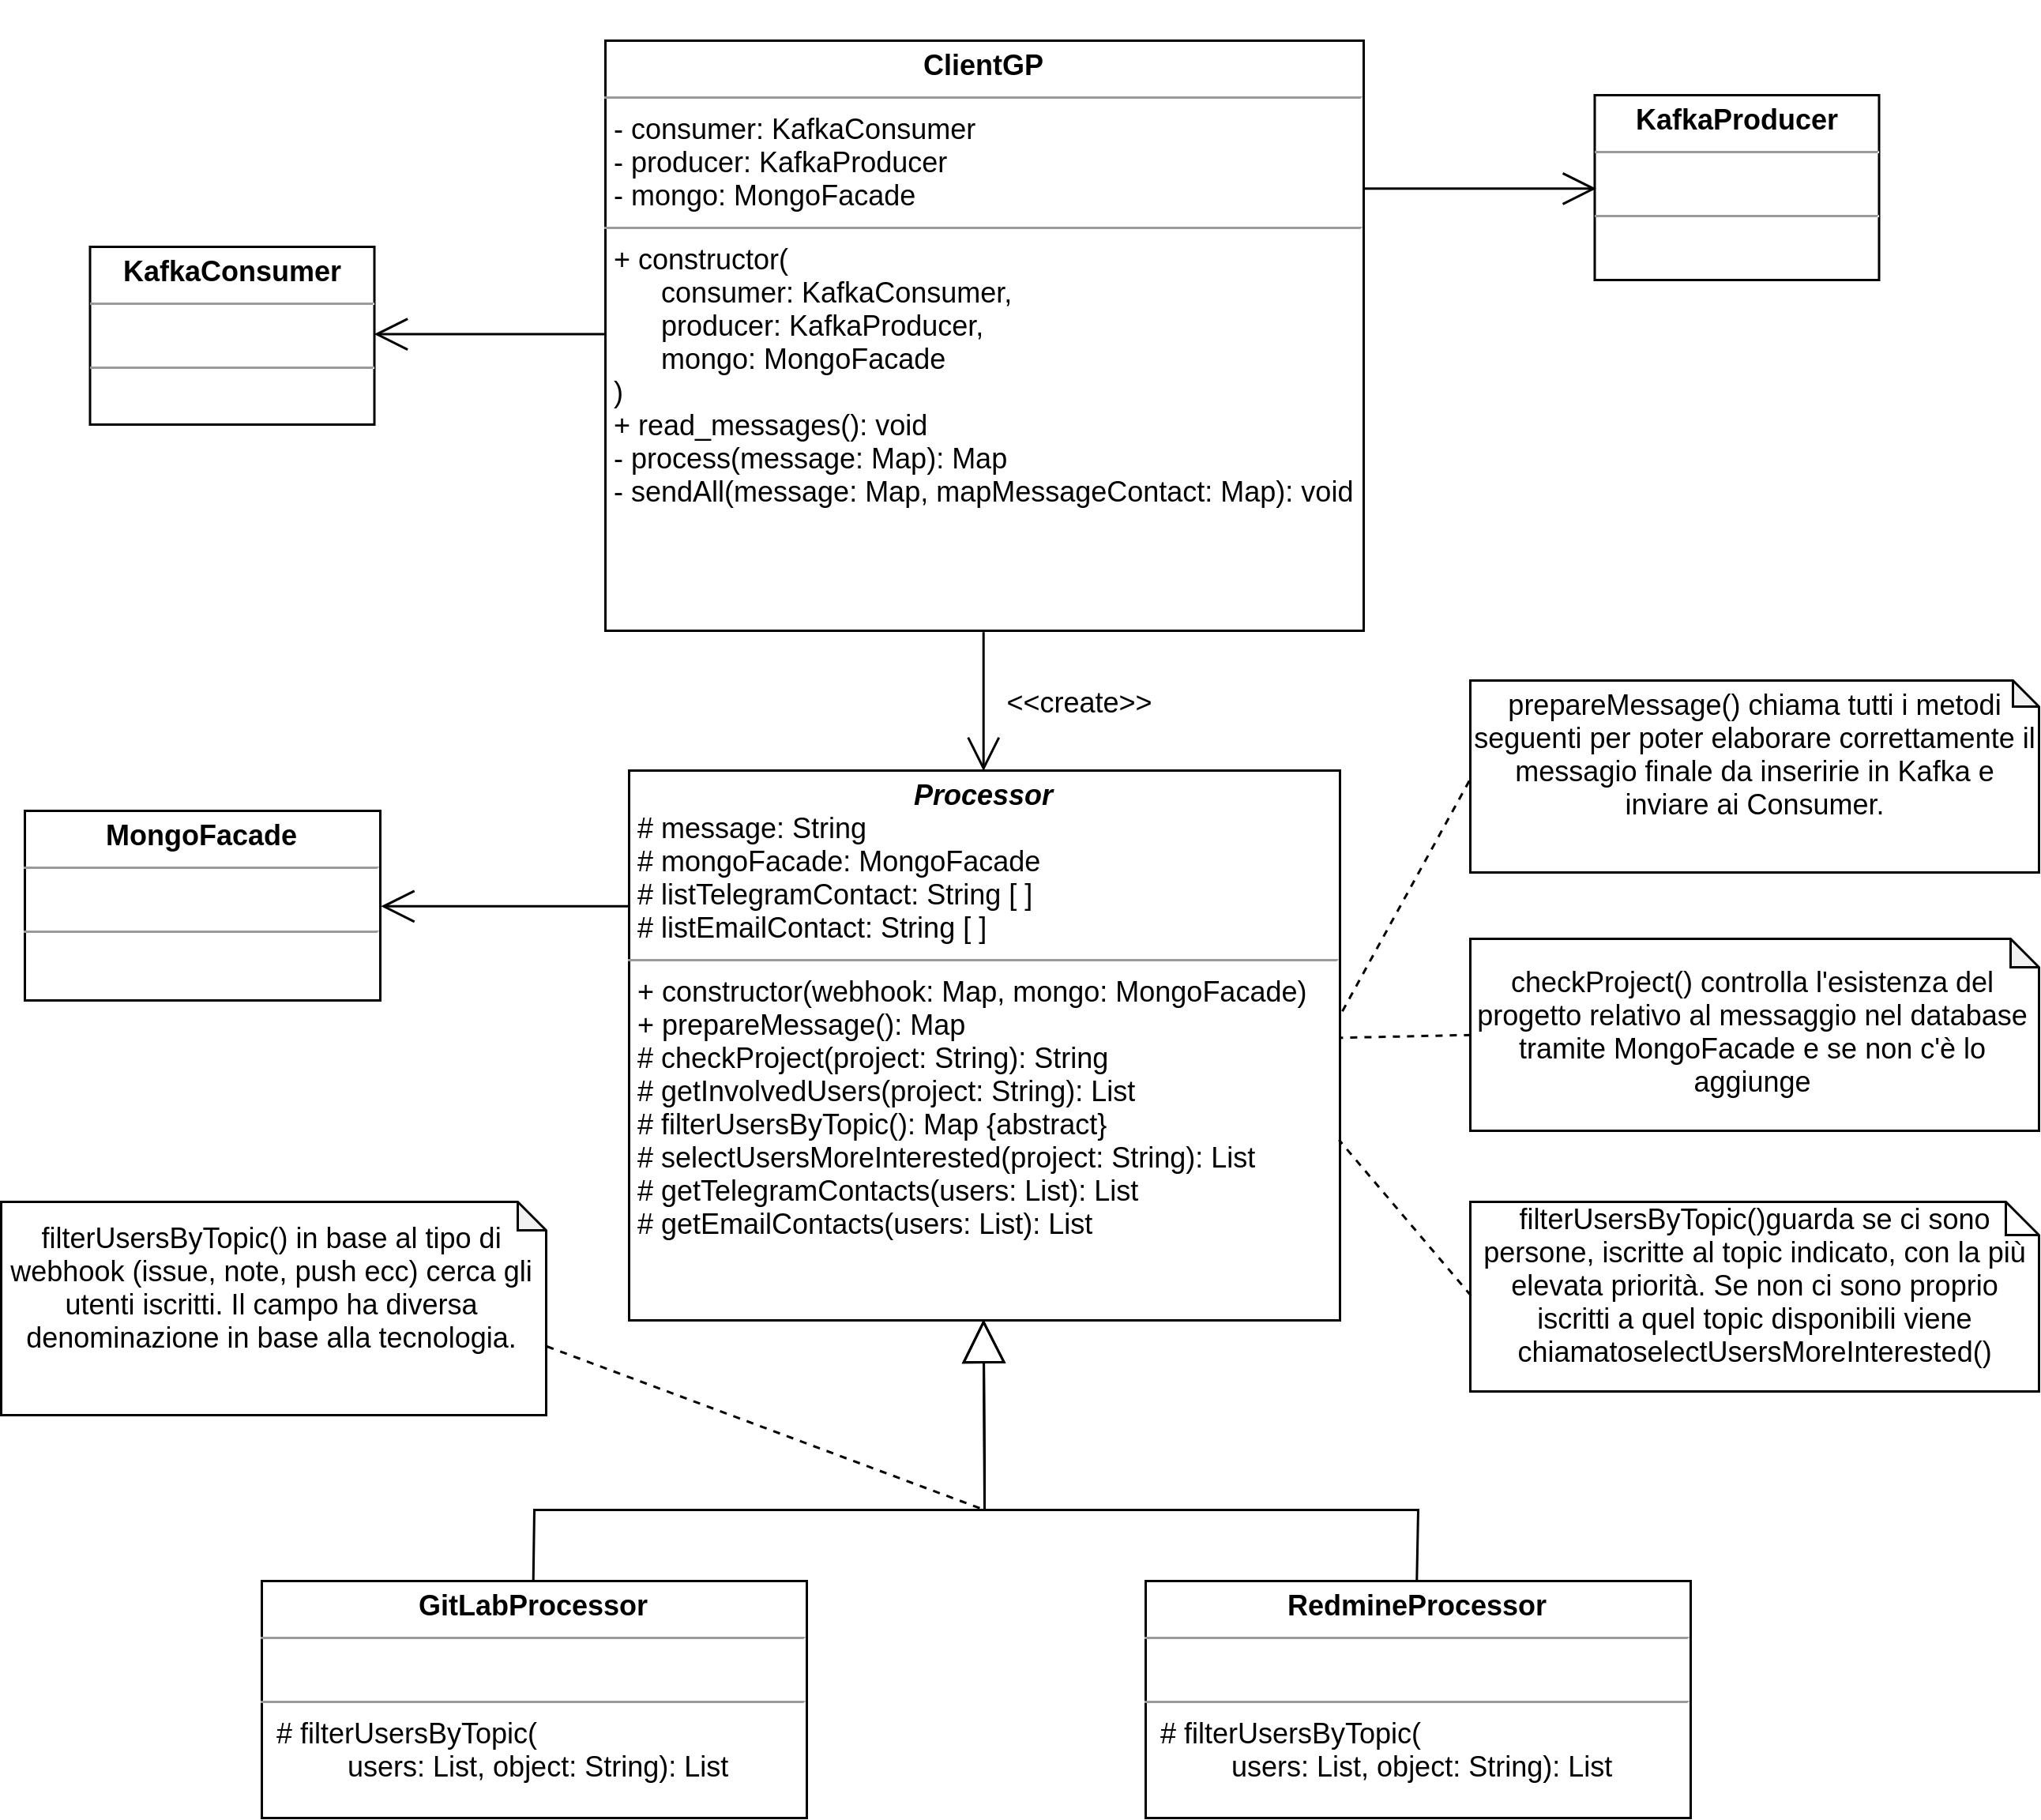
\includegraphics[width=\textwidth]{img/GP-Kafka.png}\\
    \caption{Interazione con Kafka del Gestore Personale}
    \label{fig:GP-Kafka}
\end{figure}

\subsection{Consumers}
Il Consumer è la componente finale. Esso resta in ascolto della sua coda specifica per applicativo (e.g. telegram, email).
Si occupa di inoltrare il messaggio al destinatario finale, tramite le API della piattaforma specifica.

Al momento della stesura di questo manuale, i Consumer implementati sono due:
\begin{itemize}
    \item TelegramConsumer
    \item EmailConsumer
\end{itemize}

\subsubsection{TelegramConsumer}

\paragraph{Diagramma dei package}

\begin{figure}[H]
    \centering
    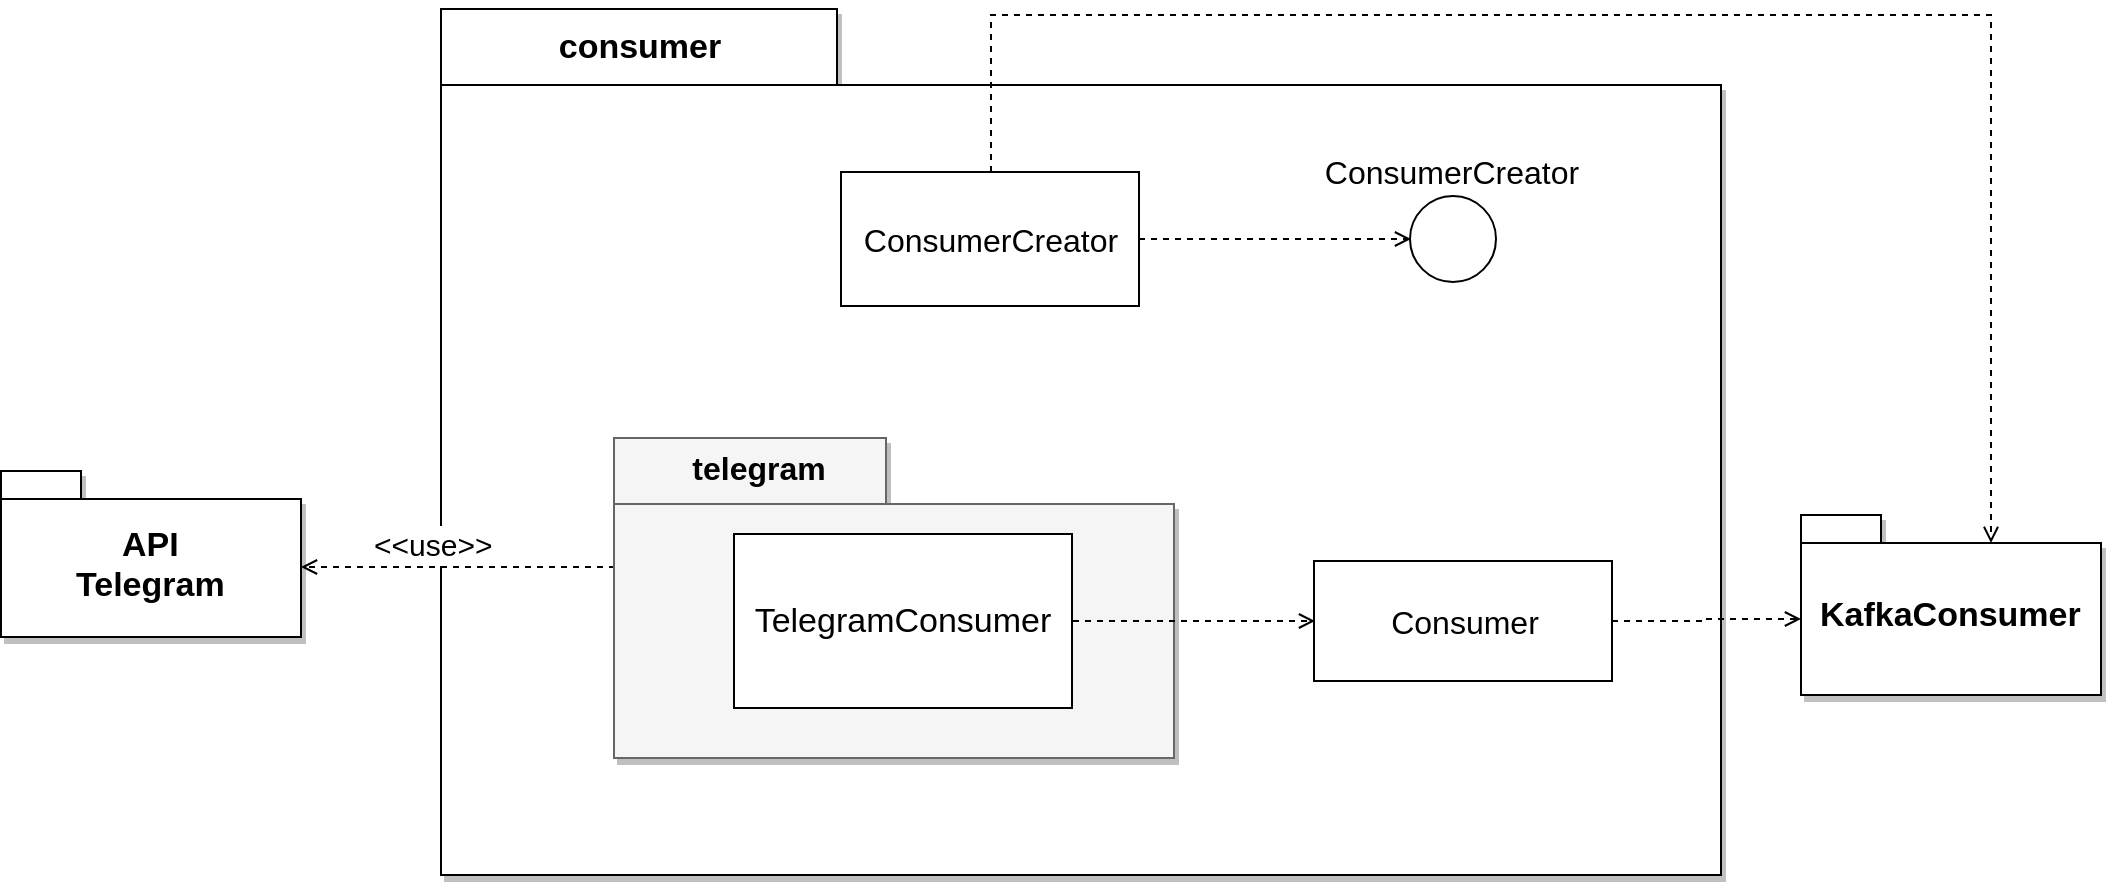
\includegraphics[width=\textwidth]{img/Package-TelegramConsumer.png}\\
    \caption{Diagramma dei package di TelegramConsumer}
    % \label{fig:GP-Kafka}
\end{figure}

\paragraph{Diagramma delle classi}

\begin{figure}[H]
    \centering
    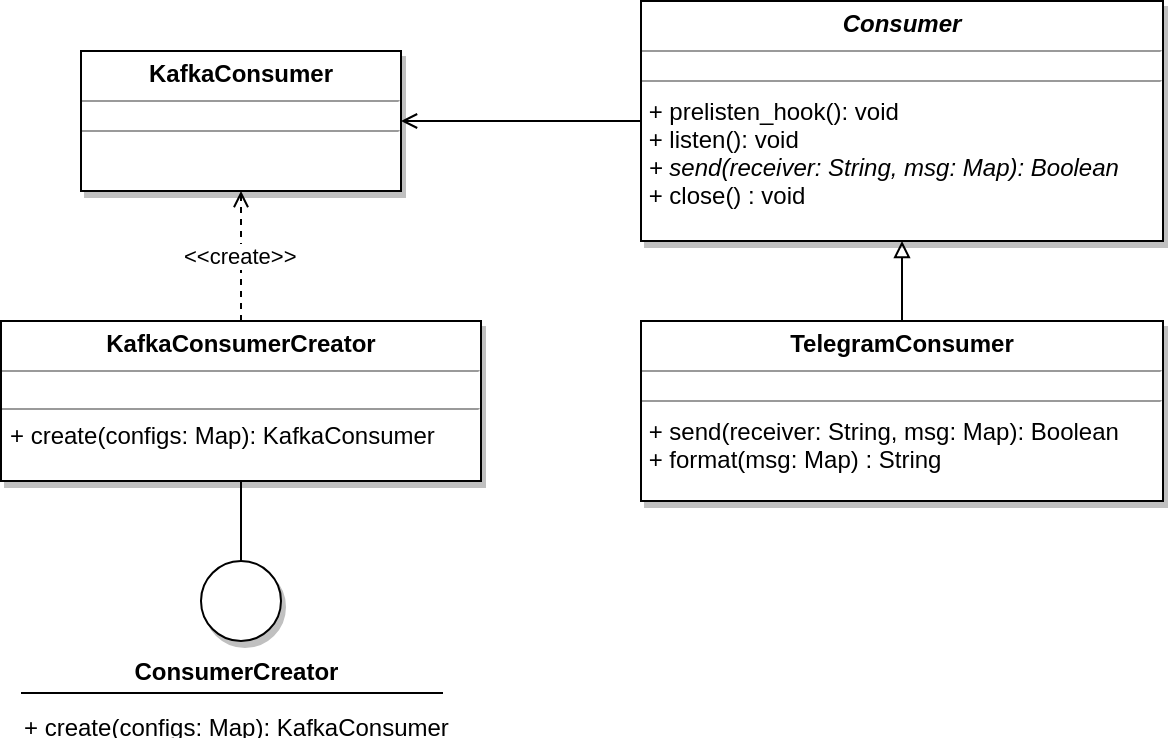
\includegraphics[width=\textwidth]{img/Consumers-TelegramConsumer.png}\\
    \caption{Diagramma delle classi di TelegramConsumer}
    % \label{fig:GP-Kafka}
\end{figure}


\subsubsection{EmailConsumer}

\paragraph{Diagramma dei package}

\begin{figure}[H]
    \centering
    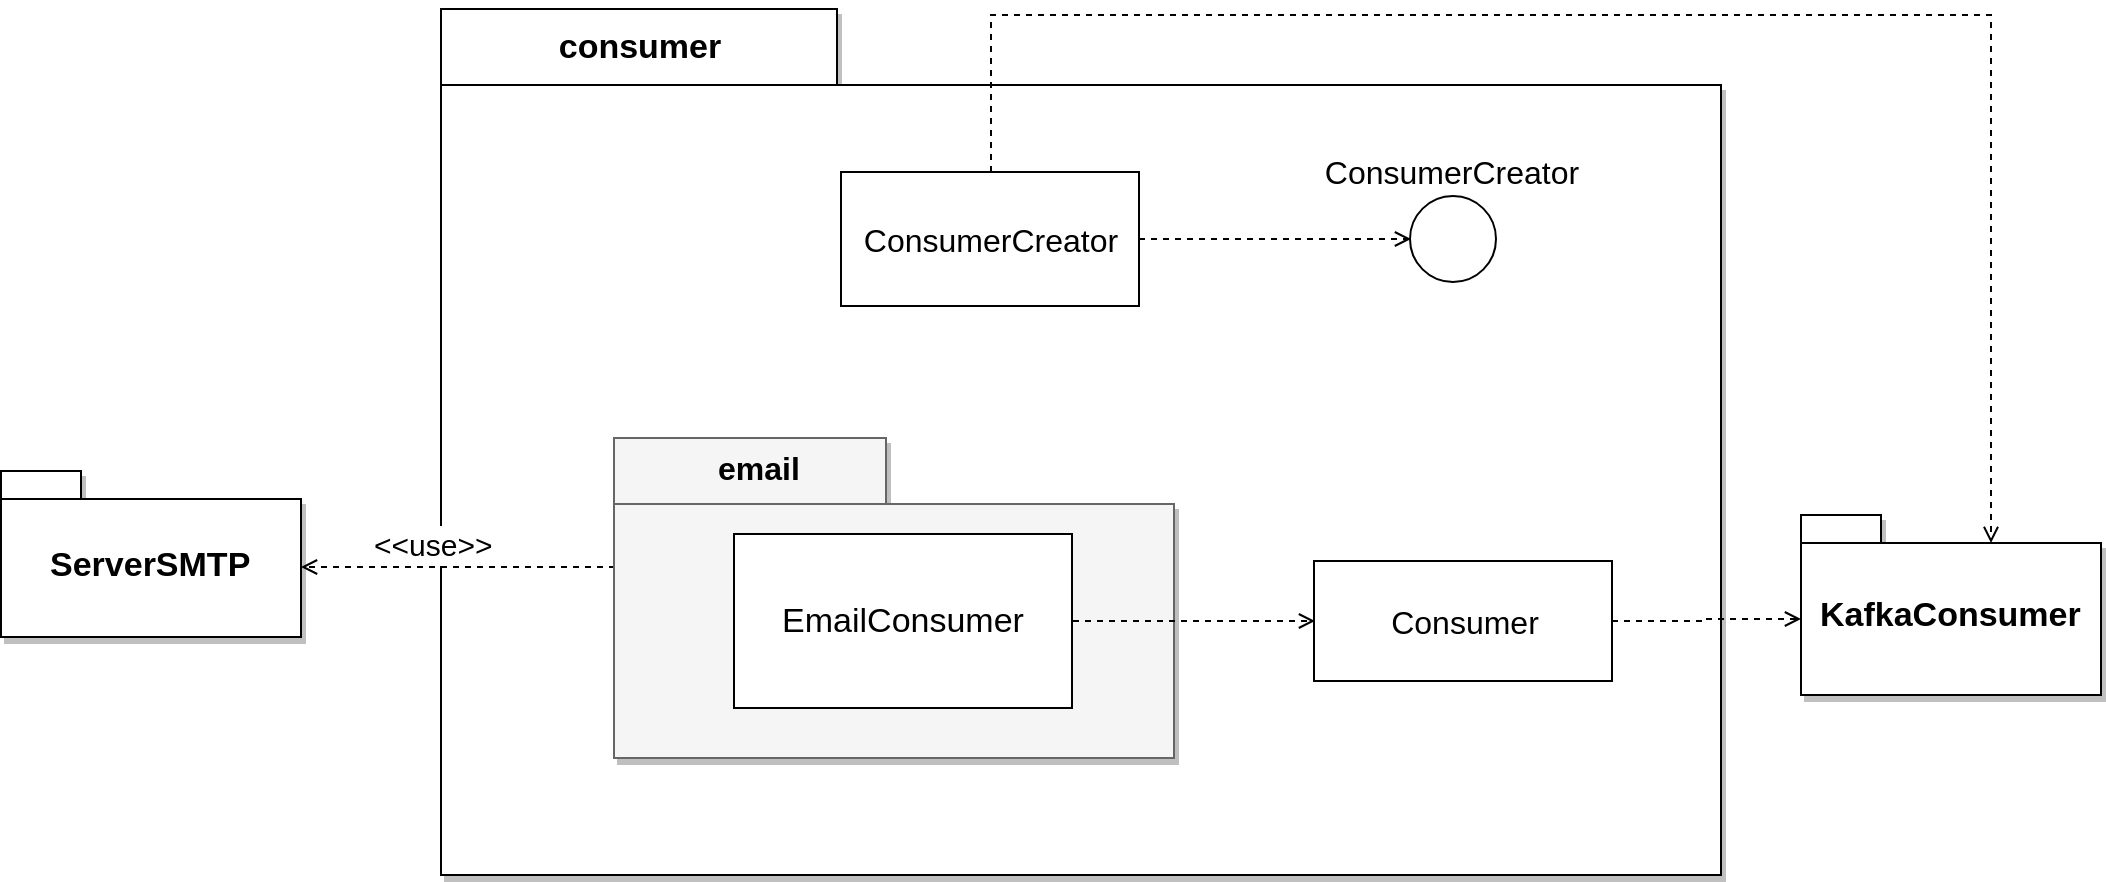
\includegraphics[width=\textwidth]{img/Package-EmailConsumer.png}\\
    \caption{Diagramma dei package di EmailConsumer}
    % \label{fig:GP-Kafka}
\end{figure}


\paragraph{Diagramma delle classi}

\begin{figure}[H]
    \centering
    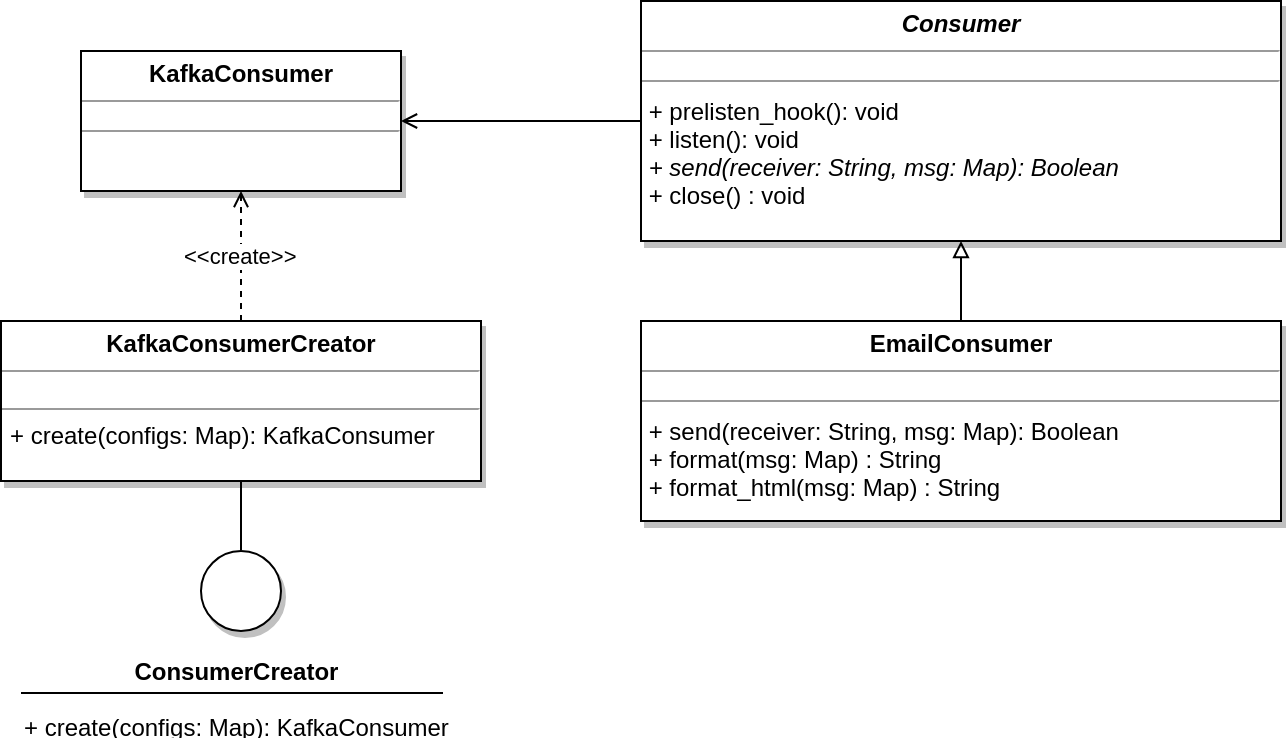
\includegraphics[width=\textwidth]{img/Consumers-EmailConsumer.png}\\
    \caption{Diagramma delle classi di EmailConsumer}
    % \label{fig:GP-Kafka}
\end{figure}


\subsection{Impostazioni dei vari componenti}

Per fare in modo che tutti i componenti vengano istanziati con i determinati parametri che permettano la giusta comunicazione tra le componenti,
ci sono dei file di configurazioni che contengono per esempio il token del bot Telegram, l'email e la password per accedere al server Email. Queste configurazioni
sono contenute nei file \texttt{``config.json''} contenuto nelle cartelle producer e consumer.

\subsection{Interazione tra i componenti}

\progetto\ vedendola ad alto livello si identificano 6 componenti. Redmine e GitLab per comunicare con i relativi Producer utilizzano dei webhook in formato JSON,
mettendosi in ascolto su determinate porte utilizzando il webserver Flask. Per quanto riguarda la comunicazione tra i Producer e Kafka utilizziamo delle istanze
di KafkaProucer. Per far comunicare Kafka con i vari Consumer utilizziamo istanze di KafkaConsumer. Nell'ultimo passo, quello che riguarda i Consumer e le applicazioni finali, quali Telegram e Email, usiamo le API messe a disposizione dagli applicativi.

\begin{figure}[H]
    \centering
    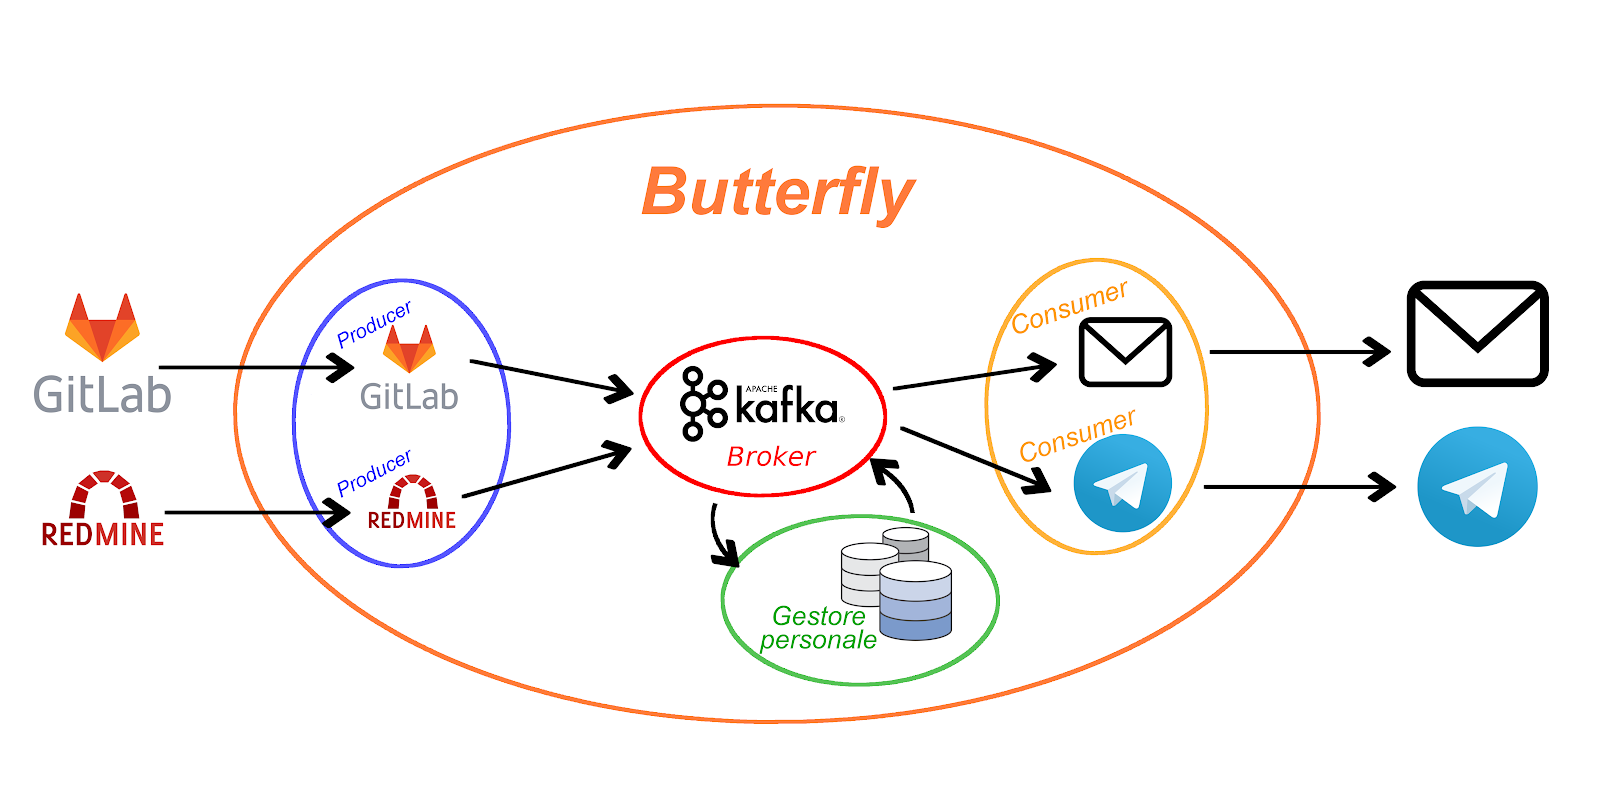
\includegraphics[width=\textwidth]{img/butterfly.png}\\
    \caption{Visione generale di \progetto}
    \label{fig:butterfly}
\end{figure}
